\documentclass{article}
\usepackage[utf8]{inputenc}
\usepackage[english]{babel}
\usepackage{mathtools}
\usepackage{amssymb}
\usepackage{rotating}
\usepackage{authblk}
\usepackage{tocloft}
\usepackage{fancyvrb}
\usepackage[titletoc]{appendix}
\renewcommand*{\cftsecdotsep}{4.5} % use dots in the section entries
\renewcommand*{\cftsecnumwidth}{3em} % increase space for Roman numerals
\renewcommand*{\cftsubsecnumwidth}{3em} % increase space for Roman numerals
\newcounter{prevpage}
\newcommand{\comment}[1]{}

% Changes for supporting info prefix "S"
% \renewcommand{\thepage}{S\arabic{page}}
% \renewcommand{\thesection}{S\arabic{section}}
% \renewcommand{\thetable}{S\arabic{table}}
% \renewcommand{\thefigure}{S\arabic{figure}}
% \renewcommand{\theequation}{S\arabic{equation}}

\usepackage[style=phys, articletitle=false, biblabel=brackets, chaptertitle=false, pageranges=false, sorting=none]{biblatex} 
\addbibresource{references.bib}

\title{
Notes on \\
\texttt{rotational-diffusion-photophysics}
}
\author[1]{Andrea Volpato} 
\affil[1]{Department of Applied Physics and Science for Life Laboratory, KTH Royal Institute of Technology, 100 44 Stockholm, Sweden}

\setcounter{Maxaffil}{0}
\renewcommand\Affilfont{\itshape\small}
\date{   }

\begin{document}
\maketitle

\clearpage
\tableofcontents

\clearpage
\listoffigures

\clearpage
%%%%%%%%%%%%%%%%%%%%%%%%%%%%%%%%%%%%%%%%%%%%%%%%%%%%%%%%%%%%%%%%%%%%%%%%%%%%%%%%
\section{Analytical models for rotational diffusion \\ and reversibly switchable states kinetics}
\label{sec:analytical_models}
In this chapter the description of polarized fluorescence experiments of photo-reactive systems in solution will be discussed. In particular we will focus our interest on fluorescence signals produced by reversible switchable fluorescent proteins (rsFPs).
We will use a rigid isotropic model for rotational diffusion, and we will assume that the diffusive properties of our system are conserved for all the species in the photo-physics kinetic scheme.  We are also assuming that the orientation of the molecule can be identified with the orientation of the transition dipole moment, which is conserved in the same orientation for every species. We are seeking an analytical solution of the diffusive problem, that is suitable for model fitting of experimental data.

%%%%%%%%%%%%%%%%%%%%%%%%%%%%%%%%%%%%%%%%%%%%%%%%%%%%%%%%%%%%%%%%%%%%%%%%%%%%%%%%
\subsection{Time evolution of orientational probabilities}
The conditional probability of a species $\epsilon$, starting with orientation $(\theta_0, \phi_0)$ at time $t=0$ from any possible species, and being at orientations $(\theta, \phi)$ at time $t$, is specified as $p_\epsilon(t,\theta,\phi|t=0,\theta_0, \phi_0)$, or for shortness $p_\epsilon(t,\theta,\phi)$. Definitions of the angles are illustrated in the sketch in figure \ref{fig:angles}.
Following the theory developed in \cite{Fisz1996a, Fisz1996b}, the time evolution of the orientational conditional probabilities can be specified using a set of differential equations as
\begin{equation}\label{eq:time_propagation}
    \frac{\partial p_\epsilon(t,\theta,\phi)}{\partial t} =
    D_R \nabla^2 p_\epsilon(t,\theta,\phi)
    + \sum_\eta k_{\epsilon\eta} (\theta,\phi) p_\eta(t,\theta,\phi),
\end{equation}
where $D_R$ is the rotational diffusion coefficient for a rigid isotropic system, $\nabla^2$ is the square gradient in the angular space, defined as
\begin{equation}
    \nabla^2 p_\epsilon(t,\theta,\phi) =
    \frac{1}{\sin(\theta)} \frac{\partial}{\partial \theta} \left(
        \sin(\theta)
        \frac{\partial p_\epsilon(t,\theta,\phi) }{\partial \theta} \right)
    + \frac{1}{\sin^2(\theta)}
    \frac{\partial^2 p_\epsilon(t,\theta,\phi) }{\partial^2 \phi},
\end{equation}
and $k_{\epsilon\eta}$ is the kinetic constant for the reaction that transform the $\eta$-th species into the $\epsilon$-th species when $\eta \neq \epsilon$, i.e. $\eta \rightarrow \epsilon$. The kinetic constant $k_{\epsilon\epsilon}$ where both indexes are the same is different than the others. It refers to the depopulation of state $\epsilon$, and it is computed summing all the possible rates that can remove population from that state
\begin{equation}\label{eq:k_diagonal}
    k_{\epsilon\epsilon}(\theta,\phi) = 
    - \sum_{\eta \neq  \epsilon} k_{\eta\epsilon}(\theta,\phi).
\end{equation}
In our problem, kinetic constants might depend on the orientation of the fluorophore, in particular this happens if the transition is induced by light-matter interaction. Moreover, in eq. \refeq{eq:time_propagation}, we can recognize two main terms: the first term models the free isotropic rotational diffusion of the system, while the second term models the kinetics and photo-physics of the system.

\begin{figure}
    \centering
    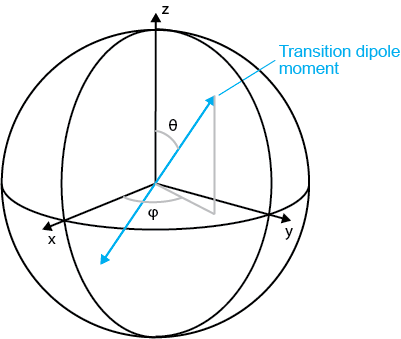
\includegraphics[width=0.5\textwidth]{figures/angles_theta_phi.png}
    \caption{Illustration of the transition dipole moment orientation and the laboratory fixed three dimensional reference frame.}\label{fig:angles}
\end{figure}

%%%%%%%%%%%%%%%%%%%%%%%%%%%%%%%%%%%%%%%%%%%%%%%%%%%%%%%%%%%%%%%%%%%%%%%%%%%%%%%%
\subsection{Spherical harmonics expansion}
All the angular functions can be expanded using a spherical harmonics (SH) basis. This approach has several advantages because SH are well behaving functions and they can simplify many aspect of the solution of the kinetic-diffusive problem. In particular the SH basis set is orthogonal and complete, and there are simple expressions to calculate products of SH functions \cite{CourantHilbertV1, Wieczorek2018}.
Orientational probabilities and kinetic constants can be expanded as
\begin{equation}\label{eq:sh_expansion}
\begin{aligned}
    p_\epsilon(t,\theta,\phi) &= \sum_{l=0}^{\infty} \sum_{m=-l}^{+l} p^{\epsilon}_{lm}(t) Y_{lm}(\theta,\phi), \\
    k_{\epsilon\eta}(\theta,\phi) &= \sum_{l=0}^{\infty} \sum_{m=-l}^{+l} k^{\epsilon\eta}_{lm} Y_{lm}(\theta,\phi)
\end{aligned}
\end{equation}
where $Y_{lm}(\theta,\phi)$ are the spherical harmonics functions of order $l$ and $m$, $p^{\epsilon}_{lm}(t)$ are the SH coefficients for the expansion of the orientational probability of state $\epsilon$, and $k^{\epsilon\eta}_{lm}$ are the coefficients for the expansion of the kinetic constants for   the $\eta \rightarrow \epsilon$ reaction.
The expansions in eq. \refeq{eq:sh_expansion} separate the angular dependence that is fully embedded in the SH basis set, from the temporal dependence in the coefficients that weight the SH basis set.
In general, if a function contains sharp angular shapes higher $l$ values will be needed to fully map its content on the SH basis set. There is an analogy with the expansion in Fourier series, in which function with higher frequency content will require higher order sinusoidal functions to be expanded completely. In this sense SH are mapping higher angular frequency content for higher $l$ values. Since the SH basis set is complete, any orientational probability can be expanded. Unconventional orientational probabilities with very sharp shapes could be achieved for example through saturation of photo-physics transitions.

Linear light-matter interaction introduces a substantial simplification on the expansion of kinetic constants of light driven processes, e.g. the transition from ground state to first excited state of a fluorophore. For all linear processes the probability of transition is proportional to the square of the scalar product of the electric field vector of radiation and the transition dipole moment of the fluorophore \cite{LakowiczBook}. This dependence directly implies that only $l=0$ and $l=2$ are involved in the expasion in eq. \refeq{eq:sh_expansion}. Moreover, if a kinetic constant does not depend on molecular orientation the expansion collapse just on the $l=0$ and $m=0$ term. Thus we can get these simplified expressions
\begin{equation}
\begin{aligned}
    k_{\epsilon\eta}(\theta,\phi) &= \sum_{l=0,2} \sum_{m=-l}^{+l} k^{\epsilon\eta}_{lm} Y_{lm}(\theta,\phi), \qquad &\text{(light-induced)} \\
    k_{\epsilon\eta}(\theta,\phi) &= k_{00}^{\epsilon\eta} \ Y_{00}(\theta,\phi) = k_{\epsilon\eta}. \qquad &\text{(orientation-independent)}
\end{aligned}
\end{equation}
Note that when using ``$4\pi$'' normalized SH functions $Y_{00}(\phi,\theta)=1$, and $k_{00}^{\epsilon\eta}=k_{\epsilon\eta}$.
This simplification greatly reduces the computation needed when solving eq. \refeq{eq:time_propagation}. If higher order light-matter interaction are present analogous simplifications are possible, e.g. two photon absorption only involve SH terms with $l=0,2,4$.

%%%%%%%%%%%%%%%%%%%%%%%%%%%%%%%%%%%%%%%%%%%%%%%%%%%%%%%%%%%%%%%%%%%%%%%%%%%%%%%%
\subsection{Solution of rigid isotropic rotational diffusion}
Spherical harmonics expansion is convenient in the context of finding a solution for rotational diffusion problems \cite{Fisz1996b}, and in particular for  isotropic rotational diffusion, i.e. the rotational diffusion of a rigid sphere without preferential axis of rotation. Spherical harmonics are eigen-functions of the rigid rotational diffusion operator, thus if we rewrite the free rotational diffusion problem in eq. \refeq{eq:time_propagation} with the expansion in eq. \refeq{eq:sh_expansion}, excluding for now the kinetics induced by photo-physics, we get
\begin{equation}\label{eq:diffusion_expansion}
\begin{aligned}
    \frac{\partial p_\epsilon(t,\theta,\phi)}{\partial t} 
    &=
    D_R \nabla^2 p_\epsilon(t,\theta,\phi) \\
    \sum_{lm}
    \frac{\partial p^\epsilon_{lm}(t)}{\partial t} Y_{lm}(\theta,\phi) 
    &=
    \sum_{lm}
        -D_R \ l(l+1) \ p^\epsilon_{lm}(t) Y_{lm}(\theta,\phi).
\end{aligned}
\end{equation}
It can be shown that to solve this set of differential equations it is only necessary to solve the differential equations on the expansion coefficients \cite{Fisz1996a}. Thus we can rewrite a new set of differential equations
\begin{equation}\label{eq:diffusion_expansion_coeffs}
    \frac{d p^\epsilon_{lm}(t)}{d t} =
    -D_R \ l(l+1) \ p^\epsilon_{lm}(t).
\end{equation}
From this set of equations we can compute the solution for the SH probability coefficients, obtaining an exponential decay of each $p^\epsilon_{lm}(t)$ coefficient starting from the initial conditions $p^\epsilon_{lm,0}=p^\epsilon_{lm}(t=0)$, 
\begin{equation}\label{eq:diffusion_solution}
    p^\epsilon_{lm}(t) =
    p^\epsilon_{lm,0} \ e^{-t/\tau_R},
\end{equation}
where the relaxation times of the diffusion terms are specified as $\tau_R = 1/D_R \ l(l+1)$. A consequence coming from this solution, and the fact that linear light-matter interaction involves only SH terms with $l=0,2$, is that free rotational diffusion of an out of equilibrium orientational state prepared in linear regime exhibits a decay time of $\tau_R = 1/D_R2(2+1) = 1/6D_R$ and a stationary component.

%%%%%%%%%%%%%%%%%%%%%%%%%%%%%%%%%%%%%%%%%%%%%%%%%%%%%%%%%%%%%%%%%%%%%%%%%%%%%%%%
\subsection{Coupling of diffusion with reversibly switchable states kinetics}
The coupling between rotational diffusion and kinetics induced by photo-physics is embedded in each kinetic contribution ``rate $\times$ population'' of eq. \refeq{eq:time_propagation}. By expanding on the SH basis set, we can greatly simplify the effort of computing the coupling of the two dynamics. Then using eq. \refeq{eq:sh_expansion} we can write
\begin{equation}\label{eq:coupling}
\begin{aligned}
    k_{\epsilon\eta} (\theta,\phi) p_\eta(t,\theta,\phi) & =
        \sum_{l_1m_1} k^{\epsilon\eta}_{l_1m_1} Y_{l_1m_1}(\theta,\phi)
        \sum_{l_2m_2} p^{\eta}_{l_2m_2}(t) Y_{l_2m_2}(\theta,\phi)
        \\
    &=
        \sum_{l_1m_1} \sum_{l_2m_2}
        k^{\epsilon\eta}_{l_1m_1}
        p^{\eta}_{l_2m_2}(t) \ Y_{l_1m_1}(\theta,\phi) Y_{l_2m_2}(\theta,\phi).
\end{aligned}
\end{equation}
Spherical harmonics have nice properties that we can exploit. In particular, since the SH basis set is complete, the product of two SH functions can be expressed as an expansion weighted by Wigner-3j coefficients \cite{AngularMomentumBook}:
\begin{equation}\label{eq:sh_product}
\begin{aligned}
    Y_{l_1m_1}(\theta,\phi) Y_{l_2m_2}(\theta,\phi) 
    =&
    \sum_{lm} \sqrt{(2l_1+1)(2l_2+1)(2l+1)} \\
    &\times
    \begin{pmatrix}
        l_1 & l_2 & l\\
        m_1 & m_2 & -m
    \end{pmatrix}
    \begin{pmatrix}
        l_1 & l_2 & l\\
        0 & 0 & 0
    \end{pmatrix}
    (-1)^{m}
    Y_{lm}(\theta,\phi),
\end{aligned}
\end{equation}
where 
$\begin{pmatrix}
    l_1 & l_2 & l\\
    m_1 & m_2 & m
\end{pmatrix}$
is a Wigner-3j coefficient. The mathematics involved in the product of spherical harmonics is formally similar to the coupling of angular momenta in quantum mechanics, where two angular momenta $l_1$ and $l_2$ are summed giving the total angular momentum $l$. In this sense part of the mathematical background is shared also when rotational diffusion and kinetics are ``summed" together.

We can rewrite the kinetic term in eq. \refeq{eq:coupling}, using eq. \refeq{eq:sh_product}, and giving
\begin{equation}\label{eq:coupling_simplified}
\begin{aligned}
    k_{\epsilon\eta} (\theta,\phi) p_\eta(t,\theta,\phi) 
    & =
    \sum_{lm} \sum_{l_2m_2} 
    k^{\epsilon\eta}_{lm,l_2m_2} p^{\eta}_{l_2m_2}(t) Y_{lm}(\theta,\phi),
    \\
\end{aligned}
\end{equation}
where we defined a new set of kinetic constants $k^{\epsilon\eta}_{lm,l_2m_2}$, that embed the algebra of the products of SH. In other words, the full description of the coupling of rotational diffusion and kinetics is found in the definition of these kinetics constants, and they can be specified as
\begin{equation}\label{eq:kinetic_sh_prod}
\begin{aligned}
    k^{\epsilon\eta}_{lm,l_2m_2}
    =&
    \sum_{l_1m_1} k^{\epsilon\eta}_{l_1m_1}
    \sqrt{(2l_1+1)(2l_2+1)(2l+1)} \\
    &\times
    \begin{pmatrix}
        l_1 & l_2 & l\\
        m_1 & m_2 & m
    \end{pmatrix}
    \begin{pmatrix}
        l_1 & l_2 & l\\
        0 & 0 & 0
    \end{pmatrix}
    (-1)^{m}.
\end{aligned}
\end{equation}
Note that the kinetic constant $k^{\epsilon\eta}_{lm,l_2m_2}$ should be interpret as the rate that connects the $l_2m_2$ SH coefficient of the orientational probability of the reagent species $\eta$ to the $lm$ SH coefficient of the orientational probability of the product species $\epsilon$. Furthermore, in this picture it is convenient to organize the set of kinetic constants $k^{\epsilon\eta}_{lm,l_2m_2}$ in a matrix $\mathbf{K}$. The two indexes of matrix elements $K_{ij}$ are meant to explore kinetic species and SH coefficients, such that $i$ indexes all the possible combinations of $(\epsilon,l,m)$ and $j$ indexes all the possible combinations of $(\eta,l_2,m_2)$. The structure of matrix $\mathbf{K}$ can also be subdivided in blocks $\mathbf{K}^{\epsilon\eta}$ that include all the terms involved in the $\eta \rightarrow \epsilon$ transition.

When the kinetics constant does not depend on the orientation of the fluorophore only the terms with $l_1=0$ and $m_1=0$ survive in eq. \refeq{eq:kinetic_sh_prod}. As a consequence the expression is simplified as
\begin{equation}
    k^{\epsilon\eta}_{lm,l_2m_2} = k_{\epsilon\eta} \ \delta_{l, l_2} \delta_{m, m_2},
\end{equation}
which implies that the kinetic block for an orientational-independent kinetic constant is diagonal and can be specified as $\mathbf{K}^{\epsilon\eta} = \mathbf{1}k_{\epsilon\eta}$ where $\mathbf{1}$ is the identity matrix.

%%%%%%%%%%%%%%%%%%%%%%%%%%%%%%%%%%%%%%%%%%%%%%%%%%%%%%%%%%%%%%%%%%%%%%%%%%%%%%%%
\subsection{Analytical solution of the full problem}
The SH expansions in eq. \refeq{eq:sh_expansion} and the kinetic term in eq. \refeq{eq:coupling_simplified} can be directly plugged in eq. \refeq{eq:time_propagation} and a new set of differential equation for the full problem is is retrieved,
\begin{equation}\label{eq:time_evoution_coeffs}
        \frac{\partial p^\epsilon_{lm}(t)}{\partial t} =
        -D_R \ l(l+1) \ p^\epsilon_{lm}(t)
        +\sum_{l_2m_2} 
        k^{\epsilon\eta}_{lm,l_2m_2} p^{\eta}_{l_2m_2}(t),
\end{equation}
that is derived analogously to eq. \refeq{eq:diffusion_expansion_coeffs}, reducing the full set of differential equations to differential equations only on the SH coefficients of the orientational probabilities.

We can collect all the rotational diffusion rates on the diagonal of matrix $\mathbf{D}$, indexed in the same way as matrix $\mathbf{K}$, such that $D_{ii} = -D_R l(l+1)$. Analogously, we can collect all the SH probability coefficients $p^\epsilon_{lm}$ in a vector $\mathbf{p}$ sharing the same indexing of matrices $\mathbf{D}$ and $\mathbf{K}$. In this way we can simplify the notation rewriting eq. \refeq{eq:time_evoution_coeffs} as
\begin{equation}
\begin{aligned}
    \frac{d \mathbf{p}(t) }{dt} &=
    \mathbf{D}\mathbf{p} + \mathbf{K}\mathbf{p} \\
    \frac{d \mathbf{p}(t)}{dt} &=
    \mathbf{M}\mathbf{p},
\end{aligned}
\end{equation}
where the matrix $\mathbf{M} = \mathbf{D} + \mathbf{K}$ collects all the rotational diffusion rates and kinetic rates. Finally, we can write the solution of this equation, in analogy to eq. \refeq{eq:diffusion_solution}, as
\begin{equation}\label{eq:full_solution}
    \mathbf{p}(t) = e^{\mathbf{M}t} \mathbf{p}_0,
\end{equation}
where $\mathbf{p}_0$ is a vector that collects all the coefficients $p^\epsilon_{lm,0}$ defining the starting conditions of the system. Note that the matrix exponential can be conveniently computed by diagonalizing matrix $\mathbf{M}$, obtaining
\begin{equation}
    e^{\mathbf{M}t} = \mathbf{U} e^{\mathbf{\Lambda} t} \mathbf{U}^{-1}, 
    \qquad \text{with} \quad
    \mathbf{M} = \mathbf{U} \mathbf{\Lambda} \mathbf{U}^{-1},
\end{equation}
where the exponential of the diagonal matrix $\mathbf{\Lambda}t$ is again a diagonal matrix with elements $e^{\Lambda_{ii}t}$, $\mathbf{U}$ is the eigenvectors matrix, and $\mathbf{\Lambda}$ is the diagonal eigenvalues matrix. From an implementation point of view, solving the full problem only requires to construct a suitable matrix $\mathbf{M}$ based on the properties of the system of interestr, and generate a suitable starting condition for the experiment, from which we will compute $\mathbf{p}_0$. The orientational probability of the fluorophores at any time delays is then promptly computed with eq. \refeq{eq:full_solution}.

The simulation of light-modulated experiments, in which laser powers are controlled with square waves, can be seen as a simple extension of the solution here proposed. The way to approach this issue it to divide the experiment in a series of time windows in which the laser powers are constant. Then for each time window a rate matrix $\mathbf{M}$ is constructed and used to propagate the probabilities. The first time window will propagate the initial conditions of the experiment, whereas the following time windows will propagate the ending conditions of the previous time window.

%%%%%%%%%%%%%%%%%%%%%%%%%%%%%%%%%%%%%%%%%%%%%%%%%%%%%%%%%%%%%%%%%%%%%%%%%%%%%%%%
\subsection{High-NA photo-selection}
The angular dependence of $k_{\epsilon\eta}$ is the way we can create a photo-selected state in which the excited molecules have a preferential orientation. If we shine light polarized along the $\hat{\mathbf{x}}$ direction of the laboratory fixed coordinate system, we can write the following expression for the kinetic constant in the low-NA limit \cite{Fisz2005}
\begin{equation}\label{eq:k_low_na}
\begin{aligned}
    k_{\epsilon\eta}(\theta,\phi)
    &= 
    | \hat{\mathbf{r}}(\theta,\phi) \cdot \hat{\mathbf{x}} |^2
    \sigma_{\epsilon\eta} \rho \\
    &=
    F_x \sigma_{\epsilon\eta} \rho
\end{aligned}
\end{equation}
where $\hat{\mathbf{r}}$ is a unitary vector pointing in the direction of the absorption transition dipole moment, $\hat{\mathbf{x}}$ is the unitary vector pointing in the direction of the electric field of the electromagnetic radiation, $F_x$ is the function encoding the pure angular dependence of the kinetic constant trough the scalar product of the two versors, $\sigma_{\epsilon\eta}$ is the cross-section for the transition $\eta\rightarrow\epsilon$ expressed in cm$^2$, and $\rho$ is the photon flux expressed in cm$^{-2}$s$^{-1}$. Cross-section and photon flux can be also expressed in terms of other widely used quantities as \cite{TkachenkoBook}
\begin{equation}
    \sigma_{\epsilon\eta} = \frac{2303}{N_A} \varepsilon,
    \qquad \text{and} \quad
    \rho = I \frac{\lambda}{h c},
\end{equation}
where $N_A$ is the number of Avogadro, $\varepsilon$ is molar extinction coefficient expressed in M$^{-1}$cm$^{-1}$, $I$ is the power density of the electromagnetic radiation expressed in W/cm$^{2}$, $\lambda$ is the wavelength, $h$ is the Planck constant, and $c$ is the speed of light.

When using high-NA objectives, eq. \refeq{eq:k_low_na} must be corrected taking in consideration the polarization mixing introduced by the focusing of the light \cite{Fisz2005}. The correction is obtained by integrating all the contribution to the excitation coming from the rays inside the focusing cone of the objective. The angle of the cone of the rays, $\alpha_0$, is obtained from the numerical aperture NA and the refractive index of the medium $n$, i.e. through the equation NA$= n\sin\alpha_0$. The corrected kinetic constant is expressed as
\begin{equation}\label{eq:high_na_k_pre}
    k_{\epsilon\eta}(\theta,\phi) =
    \left(K_a F_z + K_b F_y + K_c F_x\right)
    \sigma_{\epsilon\eta} \rho
\end{equation}
where we assumed $\hat{\mathbf{z}}$ as the propagation direction, $\hat{\mathbf{y}}$ as the perpendicular direction, and where $K_a$, $K_b$, and $K_c$ are the normalized Axelrod coefficients \cite{Fisz2005}, specified as
\begin{equation}\label{eq:high_na_k}
\begin{aligned}
    K_a &= 1/6 \ (2 - 3\cos\alpha_0 +\cos^3\alpha_0)/(1 - \cos\alpha_0)\\
    K_b &= 1/24 \ (1 - 3\cos\alpha_0 + 3\cos^2\alpha_0 -\cos^3\alpha_0)/(1 - \cos\alpha_0) \\
    K_c &= 1/8 \ (5 - 3\cos\alpha_0 - \cos^2\alpha_0 -\cos^3\alpha_0)/(1 - \cos\alpha_0). \\
\end{aligned}
\end{equation}
The correction coefficients are normalized such that $K_a + K_b + K_c = 1$, and in the low-NA limits they tend to $K_c=1$ and $K_a=K_b=0$.

%%%%%%%%%%%%%%%%%%%%%%%%%%%%%%%%%%%%%%%%%%%%%%%%%%%%%%%%%%%%%%%%%%%%%%%%%%%%%%%%
\subsection{High-NA polarized detection}
The fluorescence signal emitted by the sample and recorded from a polarized detector is derived with a similar formalism to the high-NA photo-selection correction \cite{Fisz2005}. For example, if we are observing with two cross polarized detectors, measuring the polarization along $\hat{\mathbf{x}}$ and $\hat{\mathbf{y}}$, the fluorescence signals are computed as
\begin{equation}\label{eq:highna_detection}
\begin{aligned}
    I_x(t) &= A \ \Phi_\text{fluo}^\epsilon
    \int\int 
    p_\epsilon(t,\theta,\phi) \
    \left(K_a F_z + K_b F_y + K_c F_x\right)
    \sin\theta d\theta d\phi \\
    I_y(t) &= A \ \Phi_\text{fluo}^\epsilon
    \int\int 
    p_\epsilon(t,\theta,\phi) \
    \left(K_a F_z + K_b F_x + K_c F_y\right)
    \sin\theta d\theta d\phi \\
\end{aligned}
\end{equation}
where $p_\epsilon(t,\theta,\phi)$ is the orientational probability of the fluorescent excited state, $A$ is a constant embedding all the experimental factors and the size of the sample, and $\Phi_\text{fluo}^\epsilon$ is the quantum yield of fluorescence of state $\epsilon$. Note that the constants $K_a$, $K_b$, and $K_c$ are related again to propagation direction, perpendicular direction and polarization direction respectively, as in eq. \refeq{eq:high_na_k}. We are also assuming that there is only one fluorescent state $\epsilon$. These expressions can be easily generalized for multiple fluorescent states. The integral in equations \ref{eq:highna_detection} can be easily computed exploiting the SH expansion of $p_\epsilon(t,\theta,\phi)$.

%%%%%%%%%%%%%%%%%%%%%%%%%%%%%%%%%%%%%%%%%%%%%%%%%%%%%%%%%%%%%%%%%%%%%%%%%%%%%%%%
\subsection{Four states model for negative rsFPs}
Photo-physics of rsFPs can be modeled as a 4 states system, with a ground on-state, a ground off-state, and the correspondent first excited states. The on- and off-state absorb in a different spectral region and we can use two laser with different wavelength to promote the interconversion among the states. The on-off switching happens through an excited state reaction, usually a cis-trans isomerization of the chromophore. Further processes might happen in the ground state, and in fast time-scales several intermediates can be revealed \cite{Laptenok2018, Woodhouse2020}. Usually, in green negative rsFPs the great change of spectroscopical properties happens a after a proton transfer in the ground state \cite{Nienhaus2016}.

Using the scheme in Figure \ref{fig:rsFP_kinetic_models}(a), we can specify all the kinetic constants using parameters that are commonly found in rsFP literature
\begin{equation}\label{eq:rsFP_k_4states}
\begin{aligned}
    k_{21} &= \sigma_{21}(\lambda) \rho(\lambda) \\
    k_{12} &= 1 / \tau_{\text{on}} \\
    k_{32} &= (1 / \tau_{\text{on}}) \ \Phi_{\text{on} \rightarrow \text{off}} \\
    k_{43} &= \sigma_{43}(\lambda) \rho(\lambda) \\
    k_{34} &= 1/ \tau_{\text{off}} \\
    k_{14} &= (1 / \tau_{\text{off}}) \ \Phi_{\text{off} \rightarrow \text{on}}\\
\end{aligned}
\end{equation}
where $\tau_{\text{on}}$ and $\tau_{\text{off}}$ are the lifetimes of the excited states, $\Phi_{\text{on} \rightarrow \text{off}}$ and $\Phi_{\text{off} \rightarrow \text{on}}$ are the quantum yield for the off- and on- switching processes respectively, and $\lambda$ the wavelength of the laser used to promote the ground to excited state transition.
We are assuming that the quantum yields do not depend on the wavelength of the exciting laser.

\begin{figure}
    \label{fig:rsFP_kinetic_models}
    \centering
    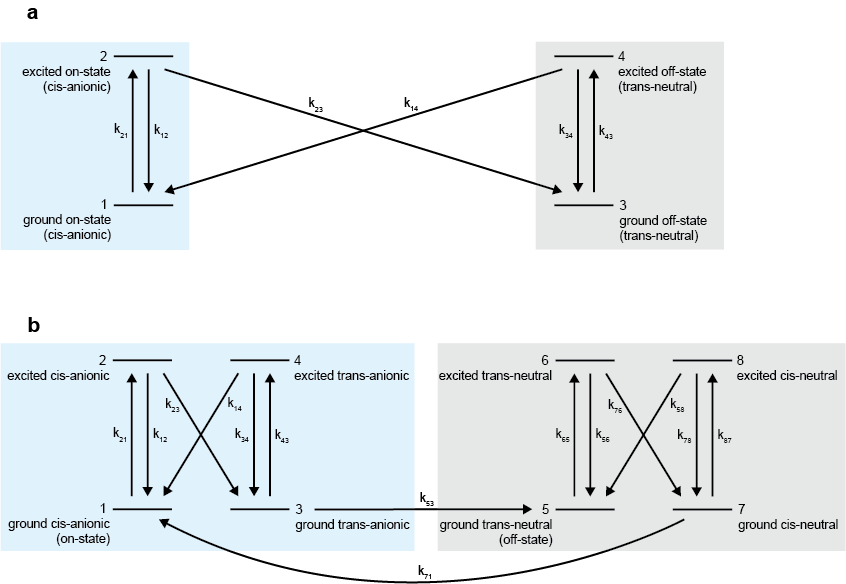
\includegraphics[width=1\textwidth]{figures/rsFP_4states_8states_kinetic_models.png}
    \caption[Kinetic models for negative rsFPs]
    {Kinetic models for negative rsFPs. (a) Four states model, and (b) eight states model. Light blue boxes highlight the anionic states, including the on-state, whereas gray boxes highlight the neutral states, which are all non-fluorescent. Fluorescence photons are emitted only from the state 2 (excited cis-anionic), when the pathway $1\rightarrow2$ is followed.}
\end{figure}

In order to implement the rsFP photo-physics in the full rotational diffusion and kinetics model, we need to compute the kinetic constants as in eq. \refeq{eq:kinetic_sh_prod}, thus we associate a block matrix $\mathbf{K}^{\epsilon\eta}$ to each kinetic rate. The block matrix include the details regarding high-NA photoselection, polarization state of the light, and the kinetic rate itself. For transitions that do not depend on the orientation of the fluorophores the block is simplified, such that $\mathbf{K}^{\epsilon\eta} = \mathbf{1}k_{\epsilon\eta} $. The block structure of the full matrix $\mathbf{K}$ can then be further specified as
\begin{equation}\label{eq:K_4states}
    \mathbf{K} =
    \begin{bmatrix}
    \square & \mathbf{K}^{12} &   & \mathbf{K}^{14} \\
    \mathbf{K}^{21} & \square \\
        & \mathbf{K}^{32} & \square  & \mathbf{K}^{34} \\
        &   &   \mathbf{K}^{43}  & \square
    \end{bmatrix}
    =
    \begin{bmatrix}
    \square & \mathbf{1}k_{12} &   & \mathbf{1}k_{14} \\
    \mathbf{K}^{21} & \square \\
        & \mathbf{1}k_{32} & \square  & \mathbf{1}k_{34} \\
        &   &   \mathbf{K}^{43}  & \square
    \end{bmatrix}.
\end{equation}
The out of diagonal matrix blocks that are missing in this expression are zeros, or in other words there are not processes that interconvert the specific couple of species. The diagonal matrix blocks, that are represented with squares $\square$ for sake of simplicity of notation, are obtained from the out of diagonal ones as in eq. \refeq{eq:k_diagonal}, e.g. $\mathbf{K}^{22} = - \mathbf{1}k_{12} - \mathbf{1}k{32}$.
Note that when multiple laser excitation are used the same species might absorb at all wavelength, and thus the corresponding kinetic matrix block will be the sum of the contributions due to different wavelengths, e.g. $\mathbf{K}^{21} = \mathbf{K}^{21}(405\text{nm}) + \mathbf{K}^{21}(488\text{nm})$. This is generally referred as crosstalk of the switching processes of rsFPs.

\subsection{Eight states model for negative rsFPs}
When the power densities employed for the switching are high enough, the excited state cis-trans isomerization might not be the rate determining step anymore. In this condition we can have the accumulation of concentration of intermediates. For example starting from the ground on-state, after the excited state flipping from cis- to trans-conformers, a protonation must occur to reach the final ground off-state. This process usually take several $\mu$s or tens of $\mu$s, and it might involve several intermediates. The simplest way to include this process in the photo-physics is to use an 8 states model. Two intermediate species are inserted between on- and off- states. The resulting scheme is represented in Figure \refeq{fig:rsFP_kinetic_models}(b).
For additional clarity, the states can be named after the conformation of the chromophore and the protonation state: cis or trans and anionic or neutral. The on-state is then also the cis-anionic state indexed with $\epsilon=1$, and the off-state is also the trans-neutral state indexed with $\epsilon=5$. The intermediate state during the off-switching process is the trans-anionic state indexed with $\epsilon=3$, whereas the intermediate state during the on-switching process is the cis-neutral state indexed with $\epsilon=7$. The excited states are respectively indexed with $\epsilon=2,4,6,\text{and }8$.
We can specify all the kinetic constants involved in this model as
\begin{equation}\label{eq:rsFP_k_8states}
    \begin{aligned}
        k_{21} &= \sigma_{\text{on}}(\lambda) \rho(\lambda) \\
        k_{12} &= 1 / \tau_{\text{on}} \\
        k_{32} &= (1 / \tau_{\text{on}}) \ \Phi^{\text{anionic}}_{\text{cis} \rightarrow \text{trans}} \\    
        k_{43} &= \sigma_{\text{on}}(\lambda) \rho(\lambda) \\
        k_{34} &= 1 / \tau_{\text{on}} \\
        k_{14} &= (1 / \tau_{\text{on}}) \ \Phi^{\text{anionic}}_{\text{trans} \rightarrow \text{cis}} \\
        k_{53} &= 1 / \tau_{\text{prot}} \\
        k_{65} &= \sigma_{\text{off}}(\lambda) \rho(\lambda) \\
        k_{65} &= 1/ \tau_{\text{off}} \\
        k_{76} &= (1 / \tau_{\text{off}}) \ \Phi^{\text{neutral}}_{\text{trans} \rightarrow \text{cis}}\\
        k_{87} &= \sigma_{\text{off}}(\lambda) \rho(\lambda) \\
        k_{78} &= 1/ \tau_{\text{off}} \\
        k_{58} &= (1 / \tau_{\text{off}}) \ \Phi^{\text{neutral}}_{\text{cis} \rightarrow \text{trans}}\\
        k_{17} &= 1 / \tau_{\text{deprot}}, \\
    \end{aligned}
\end{equation}

where $\tau_\text{prot}$ and $\tau_\text{deprot}$ are the time constants for the ground state protonation and deprotonation processes.
In this parametrization we are assuming that the absorption spectrum and the lifetimes of cis and trans species are the same. This is a reasonable assumption in negative green rsFPs \cite{Yadav2015b}, but the model can easily accept different properties for cis and trans conformers.

The full kinetic matrix is constructed in analogy to eq. \refeq{eq:K_4states} as
\begin{equation}\label{eq:K_8states}
    \mathbf{K} = 
    \begin{bmatrix}
    \square & \mathbf{1}k_{12} &  & \mathbf{1}k_{14} & & & \mathbf{1}k_{17}  \\
    \mathbf{K}^{21} & \square \\
    & \mathbf{1}k_{32} & \square  & \mathbf{1}k_{34} \\
    & & \mathbf{K}^{43}  & \square \\
    & & \mathbf{1}k_{53} &  &  \square & \mathbf{1}k_{56} & & \mathbf{1}k_{58} \\
    & & & & \mathbf{K}_{65} & \square \\
    & & & & & \mathbf{1}k_{76} & \square & \mathbf{1}k_{78} \\
    & & & & & & \mathbf{K}_{87} & \square 
    \end{bmatrix}.
\end{equation}
Note that $\mathbf{K}^{21} =  \mathbf{K}^{43}$ and $\mathbf{K}^{65} =  \mathbf{K}^{87}$ because we are assuming the same absorption cross-sections for cis-anionic/trans-anionic states and trans-neutral/cis-neutral states respectively.

%%%%%%%%%%%%%%%%%%%%%%%%%%%%%%%%%%%%%%%
\subsection{Parametrization of rsEGFP2}\label{sec:rs2_parametrization}
The parametrization of the reversible switchable protein rsEFGP2 was mainly derived from \cite{Khatib2016}.
In particular, the absorption properties of the on-state and off-state can be specified with the extinction coefficients \cite{Khatib2016},
\begin{equation}
    \begin{aligned}
        \epsilon_{\text{on}} (488 nm) &= 51560 \ \text{M}^{-1} \text{cm}^{-1} \\
        \epsilon_{\text{on}} (405 nm) &= 5260 \ \text{M}^{-1} \text{cm}^{-1} \\
        \epsilon_{\text{off}} (488 nm) &= 60 \ \text{M}^{-1} \text{cm}^{-1} \\
        \epsilon_{\text{off}} (405 nm) &= 22000 \ \text{M}^{-1} \text{cm}^{-1} \\
    \end{aligned}
\end{equation}
and then the cross-sections $\sigma$ in cm$^2$ can be computed accordingly using the equation \cite{TkachenkoBook}
\begin{equation}
    \sigma(\lambda) = \frac{2303}{N_A}\epsilon(\lambda),
\end{equation}
where $N_A$ is the Avogadro number.
The quantum yields of fluorescence and cis-trans isomerization are as follows \cite{Khatib2016}
\begin{equation}
    \begin{aligned}
        \Phi_\text{fluo} &= 0.35 \\
        \Phi^{\text{anionic}}_{\text{cis} \rightarrow \text{trans}} &= 1.65 \cdot 10^{-2} \\
        \Phi^{\text{neutral}}_{\text{trans} \rightarrow \text{cis}} &= 0.33. \\
    \end{aligned}
\end{equation}
The fluorescence lifetimes are $\tau_\text{on} = 1.6$ ns \cite{Testa2015} and $\tau_\text{off} \approx$ ps \cite{Woodhouse2020} (20 ps are assumed). Finally $\tau_\text{deprot} = 5.1$ us, in agreement to dynamics observed in transient absorption measurements \cite{Woodhouse2020}, and $\tau_\text{prot} = 48$ $\mu$s was determined from high-power off-switching data, see section \ref{sec:high_power_offswitching}.
The absorption properties of cis and trans conformers of the same protonation state were taken as equal, i.e. $\epsilon_\text{on}(\lambda) = \epsilon_\text{cis}^\text{anionic}(\lambda) \approx \epsilon_\text{trans}^\text{anionic}(\lambda)$ and $\epsilon_\text{off}(\lambda) = \epsilon_\text{trans}^\text{neutral}(\lambda) \approx \epsilon_\text{cis}^\text{neutral}(\lambda)$. This is a reasonable approximation given the fact that the absorption spectra are very close, see supporting information of \cite{Woodhouse2020}.

Two remaining parameters are undefined, $\Phi^{\text{anionic}}_{\text{trans} \rightarrow \text{cis}}$ and $\Phi^{\text{neutral}}_{\text{cis} \rightarrow \text{trans}}$. These quantum yields enable the back-conversion from the intermediate states. $\Phi^{\text{anionic}}_{\text{trans} \rightarrow \text{cis}}$ will be fitted in section \ref{sec:starss2_fit}, whereas $\Phi^{\text{neutral}}_{\text{cis} \rightarrow \text{trans}}$ will be assumed as 0. Assuming a null quantum yield silences the associated process. This is a reasonable assumption if there is not an accumulation of intermediate in the on-switching process that is excited with 405 nm light. Further characterization will be needed to better characterize the back-conversion quantum yields.


\clearpage
%%%%%%%%%%%%%%%%%%%%%%%%%%%%%%%%%%%%%%%%%%%%%%%%%%%%%%%%%%%%%%%%%%%%%%%%%%%%
% \section{Simulation of STARSS experiments}
% Three experiments exploiting STARSS with long-lived states were proposed in the main manuscript. In this section we will simulate examples using the analytical model. This will allow to gain insight on state populations and to grasp a deeper understanding of the experimental observables.
\section{STARSS method 1 simulation of experiments}\label{sec:starss_modality1}
In STARSS method 1 experiments, a short pulse (about 250 ns) of polarized laser light at 405 nm is shined on a sample containing rsFPs. This induces the on-switching of a pool of fluorophores that are roughly oriented with the electric field of the light. The linear photo-selection process generates a ``cos$^2$'' orientational probability distribution of on-switched molecules. Light-matter interaction limits the precision/sharpness of the orientational probability distribution that can be created. Additionally, high-NA objectives limit the degree of alignment of the on-switched pool of molecules because they introduce electric field components of the light in all dimensions, i.e. small components along Y and Z even if the direction of polarization of the beam is along X.

% Pulse scheme
\begin{figure}[h!]
    \centering
    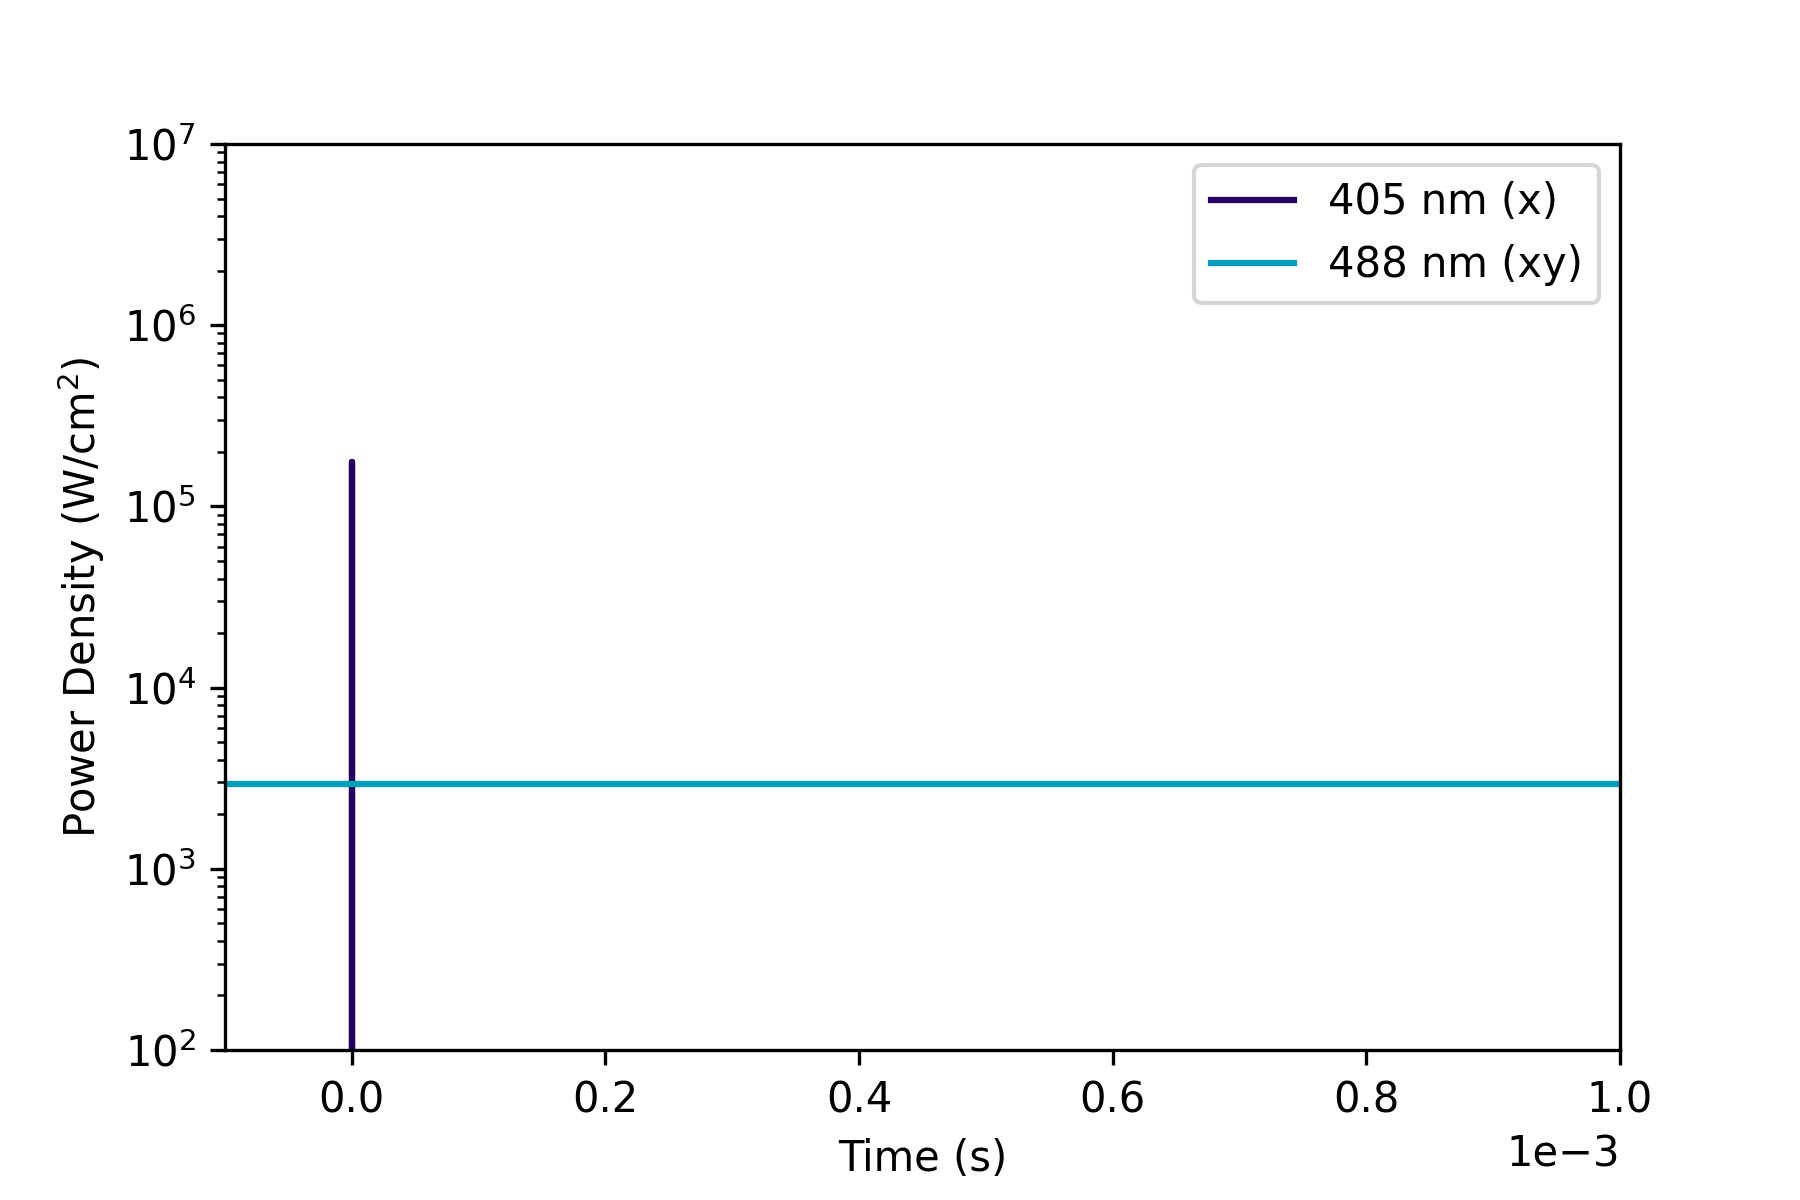
\includegraphics[width=0.8\textwidth]
    {figures/starss1_pulse_scheme.png}
    \caption[Power density used in the simulation of STARSS method 1]
    {Power density of laser beams used in the simulation of STARSS with long-lived states method 1. The duration of the high power burst of 405 nm light is 250 ns. The circularly polarized 488 nm beam is kept on during the full duration of the pulse scheme.}
    \label{fig:starss1_pulse_scheme}
\end{figure}

At the beginning of the pulse scheme of this experiment the rsFPs are kept in the off-state by shining 488 nm light. The signal is not exactly zero because of the crosstalk between the on- and off-switching process, i.e. there is a small chance of on-switching the rsFPs using 488 nm light. After delivering the short high-power burst of 405 nm light, a fraction of rsFPs start the on-switching process. We can assume that the cis-trans conformational change, which is happening in the excited state, is instantaneous compared to the time-scale of the experiment. After the conformational change the rsFP chromophore is still not fluorescent, and a deprotonation in the ground state must happen in order to maturate the final fluorescent on-state (cis-anionic).
The deprotonation process affects the data and generates an exponential rise of the fluorescence signal with a time scale of roughly 5 $\mu$s. For the simulation we used 5.1 $\mu$s which is the time scale observed in transient spectroscopy experiments \cite{Woodhouse2020}. 
As soon as the proton transfer happens, there is a big shift of absorption properties of the rsFP chromophore. In the cis-anionic state there is a high probability of absorbing 488 nm photons, which can immediately trigger off-switching events. The competition of the maturation of the on-switching and the start of the off-switching generates fluorescence signals with a rise and then a decay, as shown in Figure \ref{fig:starss1_signal}.
The mismatch between the detectors is induced by the on-switching photo-selection that lasts as long as the characteristic rotational diffusion time for the system. Note that repeating the same experiment with circularly polarized 405 nm light gives two identical signals in the cross-polarized detectors.

% Detectors signal
\begin{figure}[h!]
    \centering 
    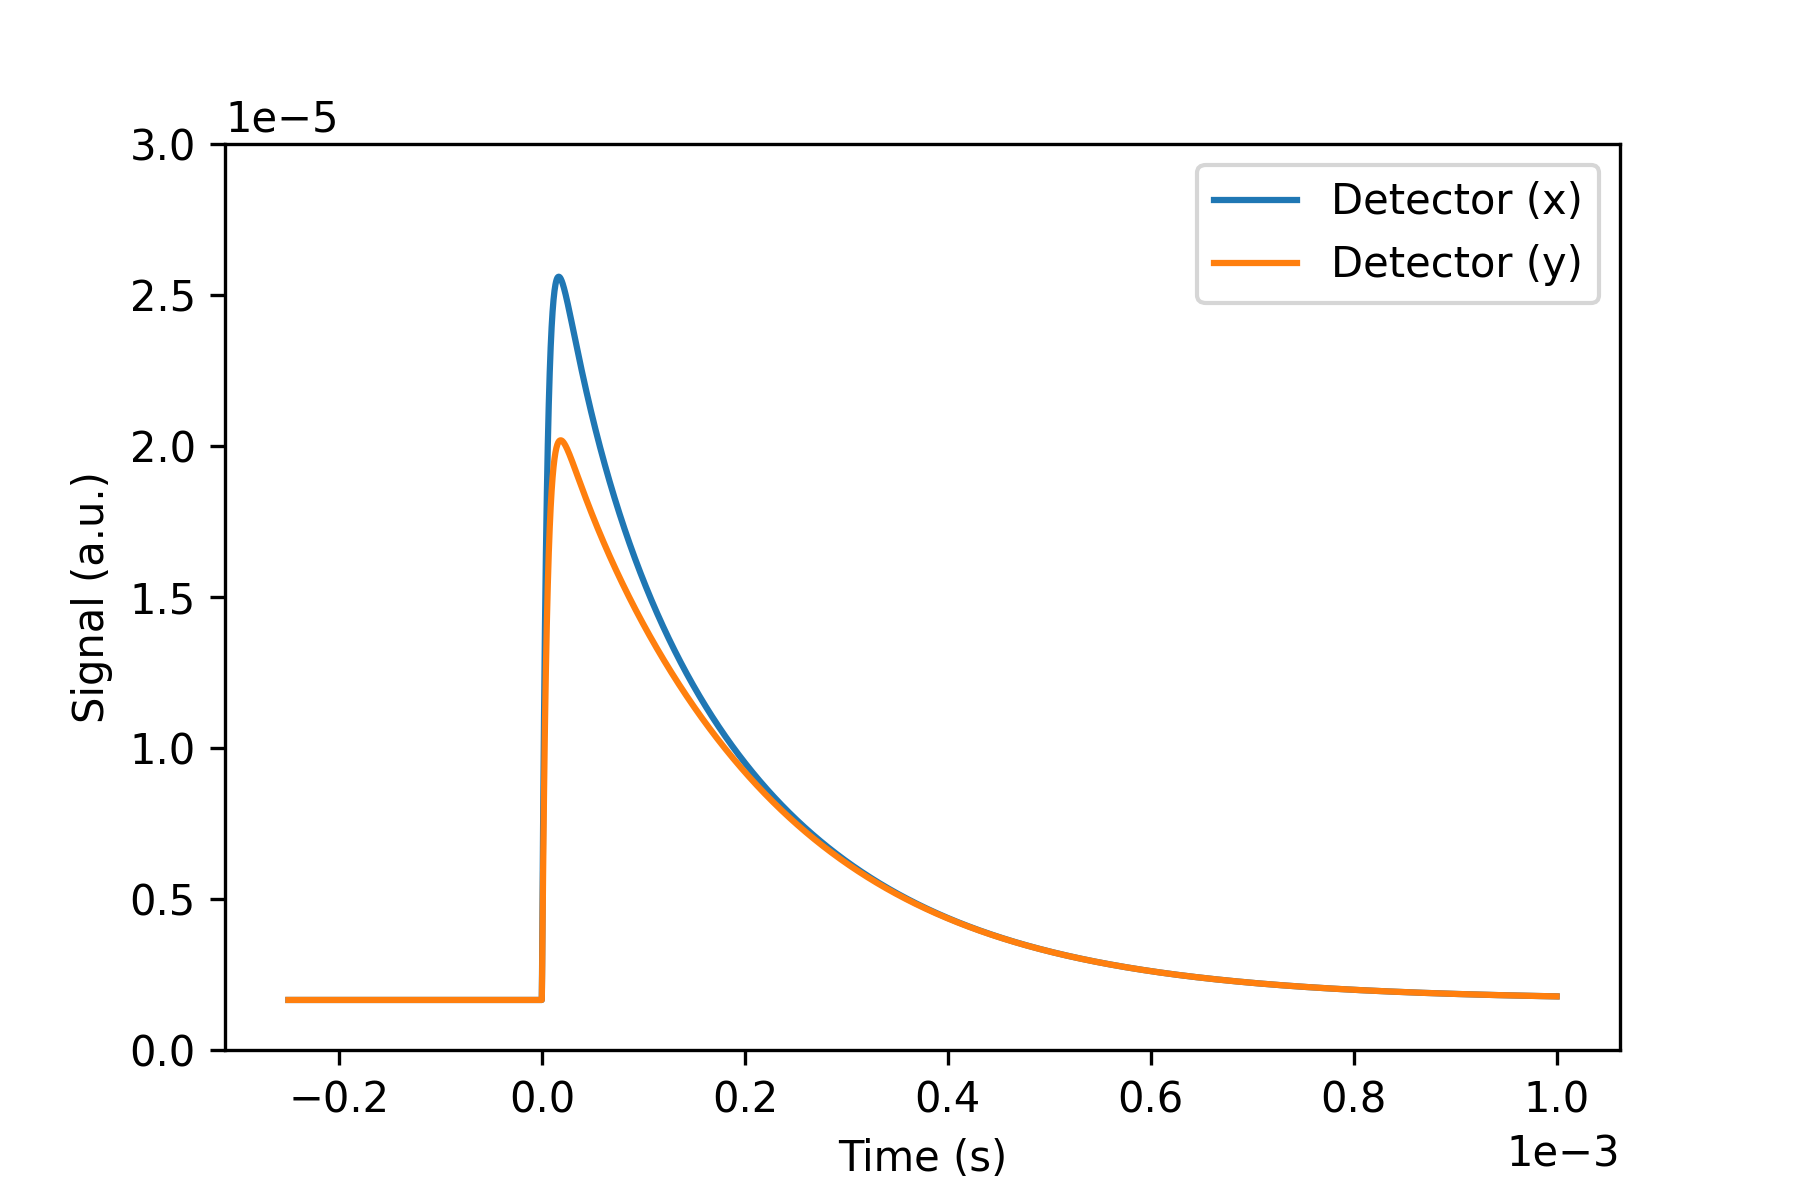
\includegraphics[width=0.8\textwidth]
    {figures/starss1_signal.png}
    \caption[Simulated detector signals of STARSS method 1]
    {Detector signals for parallel (x) and perpendicular (y) channels in the simulation of STARSS with long lived states method 1. The rotational diffusion time in this simulated experiment is 100 $\mu$ and the fluorophore is rsEFGP2 with parameters presented in Section \ref{sec:rs2_parametrization}.}
    \label{fig:starss1_signal}
\end{figure}

The on- and off-switching processes, inevitably coupled to the fluorescence readout of rsFPs, affect the experiments but do not sensibly modify the typical exponential decay observed in traditional time-resolved fluorescence anisotropy experiments. The simulated decay traces in Figure \ref{fig:starss1_anisotropy} (blue lines) are well approximated by a mono-exponential decay where the observed decay constant coincides with the rotational diffusion time (dashed orange lines). This suggests that we can borrow the traditional theory of time-resolved fluorescence anisotropy experiments \cite{LakowiczBook} to extract the rotational diffusion coefficient and compute an estimate for the Stokes radius of the system labeled with rsFPs.

The main deviations from the mono-exponential behaviour are located at later times where slow rotational diffusive samples are faster than predicted with mono-exponential behavior. Fast rotational diffusive samples have a slight bi-exponential behavior with an additional small-amplitude fast component of anisotropy. Nevertheless, there is a clear time window where blue and orange curves superimpose almost perfectly. When the off-switching process is almost completed (after a few hundreds of $\mu$s) the reactivation induced by circularly polarized 488 nm light adds a slow depolarization mechanism. This effect shortens the anisotropy decay when the rotational diffusion time is much slower than the off-switching time constant.
In the simulated conditions and for the time window at ~2-500 $\mu$s, the anisotropy traces are in good agreement with the mono-exponential signal expected from a standard time-resolved florescence anisotropy experiment. Note that slowing down the off-switching process by reducing the power density of the 488 nm light, can extend this window to much slower decays, at the cost of reducing the fluorescence counts.


% Anisotropy
\begin{figure}[h!]
    \centering
    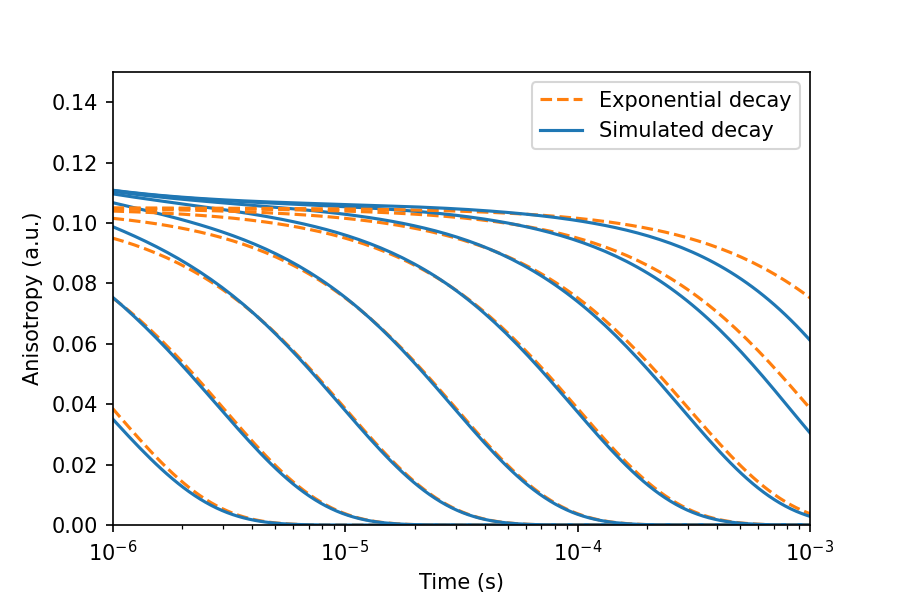
\includegraphics[width=0.8\textwidth]
    {figures/starss1_anisotropy_exponential_decays.png}
    \caption[Simulated fluorescence anisotropy decays of STARSS method 1]
    {Fluorescence anisotropy decays computed for rsEFGP2 labeled systems in the simulation of STARSS with long lived states method 1 with rotational diffusion times of 1, 3, 10, 30, 100, 300, 1000, 3000 $\mu$s starting from left to right, respectively. Anisotropy is computed from similar curves to the ones presented in Figure \ref{fig:starss1_signal}, using the anisotropy equation and by subtracting the residual steady-state background obtained at infinity when the off-switching is considered completed.}
    \label{fig:starss1_anisotropy}
\end{figure}

The starting value $r_0$ of an anisotropy decay could theoretically start from a maximum value of 0.4, when linear photo-selection is involved. In a more realistic system several factors can diminish $r_0$.
The rotation of the emission transition dipole moment with respect to the absorption transition dipole moment is a source of anisotropy loss. In green rsFPs, where a cis-trans isomerization is involved, the angle between the absorption transition dipole moment of the off-species and the emission transition dipole moment of the on-species is about $\alpha=30$-$35^\circ$ \cite{Yadav2015}. This induces a reduction of the maximum anisotropy to $r_0 = (3 \cos^2 \alpha -1)/5 \approx 0.32$-$0.29$ \cite{LakowiczBook}.
Additional losses of anisotropy arise from: (i) saturation of photo-selected states, that happens when the on-switched fraction is much higher than 10\% (this could be used to increase the fluorescence photon counts); (ii) high-NA photo-selection and detection that mixes the polarization of the excitation light and the detection collection efficiency, thus reducing the maximum difference that can be measured between the detectors; and (iii) fast local mobility of the probe, that introduces anisotropy decay components that are lost in sub-microsecond timescales.
The simulation proposed here includes all the effects that couple on- and off-switching processes to the losses of anisotropy, and also high-NA effects. Rotation of the transition dipole moments and a modelling of diffusion at fast local mobility are not included, but they will be the subjects of future studies.

% % Anisotropy
% \begin{figure}[h!]\label{fig:starss1_anisotropy}
%     \centering
%     \includegraphics[width=0.8\textwidth]
%     {figures/starss1_anisotropy.png}
%     \caption{fluorescence anisotropy decay computed from signals in Figure \ref{fig:starss1_signal}.}
% \end{figure}

% Sphere series
\begin{figure}[h!]
    \centering
    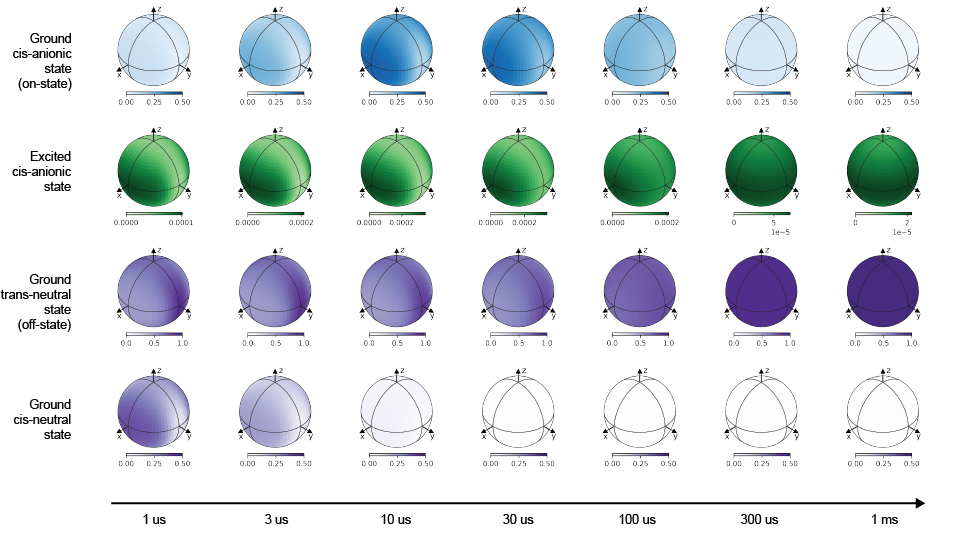
\includegraphics[width=1\textwidth]
    {figures/starss1_spheres_time_axis.png}
    \caption[Time evolution of orientational probabilities for STARSS method 1]
    {Time evolution of orientational probabilities of ground cis-anionic state (blue), excited cis-anionic state (green), ground trans-neutral state (purple, top), and ground cis-neutral state (purple, bottom) for STARSS method 1. The rotational diffusion time in this simulated experiment is 100 $\mu$s and the fluorophore is rsEFGP2.}
    \label{fig:starss1_sphere_series}
\end{figure}

The experiment can be followed best by exploring the time evolution of the orientational probabilities of the states involved in the kinetics of on- and off-switching. At the beginning of the experiment the system is prepared in a way such that almost all the fluorophores are in the off-state. After on-switching with a 405 nm laser pulse, a fraction of the fluorophores with the transition dipole moment aligned along X is converted from the trans-neutral to the cis-neutral state. In a few microseconds, the cis-neutral chromophores convert spontaneously to the cis-anionic (on-) state. This process generates a rise in the fluorescence signal, that is polarized if the rotational diffusion of the fluorescently labeled system is slow enough. If slow rotational diffusion is present the excited cis-anionic state population distribution resembles the one of the photo-selected state, i.e. the green distribution in figure \ref{fig:starss1_sphere_series} resemble the purple distribution in the last row at early times. As the rotational diffusion evolves, the excited cis-anionic state population loses the polarized shape and becomes symmetric along x and y. At the same time the off-switching process, which for negative switchers is coupled to the readout, decreases the total population of the cis-anionic state, reaching again the initial condition of the experiment.
\clearpage


\clearpage
%%%%%%%%%%%%%%%%%%%%%%%%%%%%%%%%%%%%%%%%%%%%%%%%%%%%%%%%%%%%%%%%%%%%%%%%%%%%%%%%%
\section{STARSS method 2 simulation of experiments}\label{sec:starss_modality2}
In STARSS with long-lived states methods 2, circularly polarized 405 nm laser light is used to activate a pool of molecules without preferential orientation along X or Y directions. A waiting time of 500 $\mu$s is used to let all the on-switching processes to be completed. The length of the waiting time also allows for the completion of slow relaxations of the fluorophore, which have been observed in transient absorption experiments \cite{Laptenok2018, Woodhouse2020}.
After on-switching, an X-linearly polarized 488 nm pulse is used to preferentially off-switch the molecules aligned with the electric field. Rotational diffusion will remove off-switched rsFPs from the X orientation, and it will repopulate the same orientation with on-switched rsFPs.

The competition of the diffusion and the off-switching processes strongly influences the fluorescence signals measured in the two detector channels. In particular, if rotational diffusion is the fast dominant dynamics, the anisotropy will stay high and constant during the full length of the experiment. In contrast, if the off-switching kinetics is competitive or faster than rotational diffusion, there will be a decay of the fluorescence anisotropy signal. The loss of anisotropy is due to a completely different phenomenon than in STARSS method 1, and negative values are also possible. This decay is due to a loss of on-switched fluorophores aligned along the parallel detection channel. With slow rotational diffusion these molecules are not exchanged for fresh ones, and a loss of signal in the parallel channel builds up. In the limit of extremely slow rotational diffusion, there could be an almost complete off-switching along the direction of the parallel channel, and negative anisotropy values are obtained.

% Pulse scheme
\begin{figure}[h!]
    \centering
    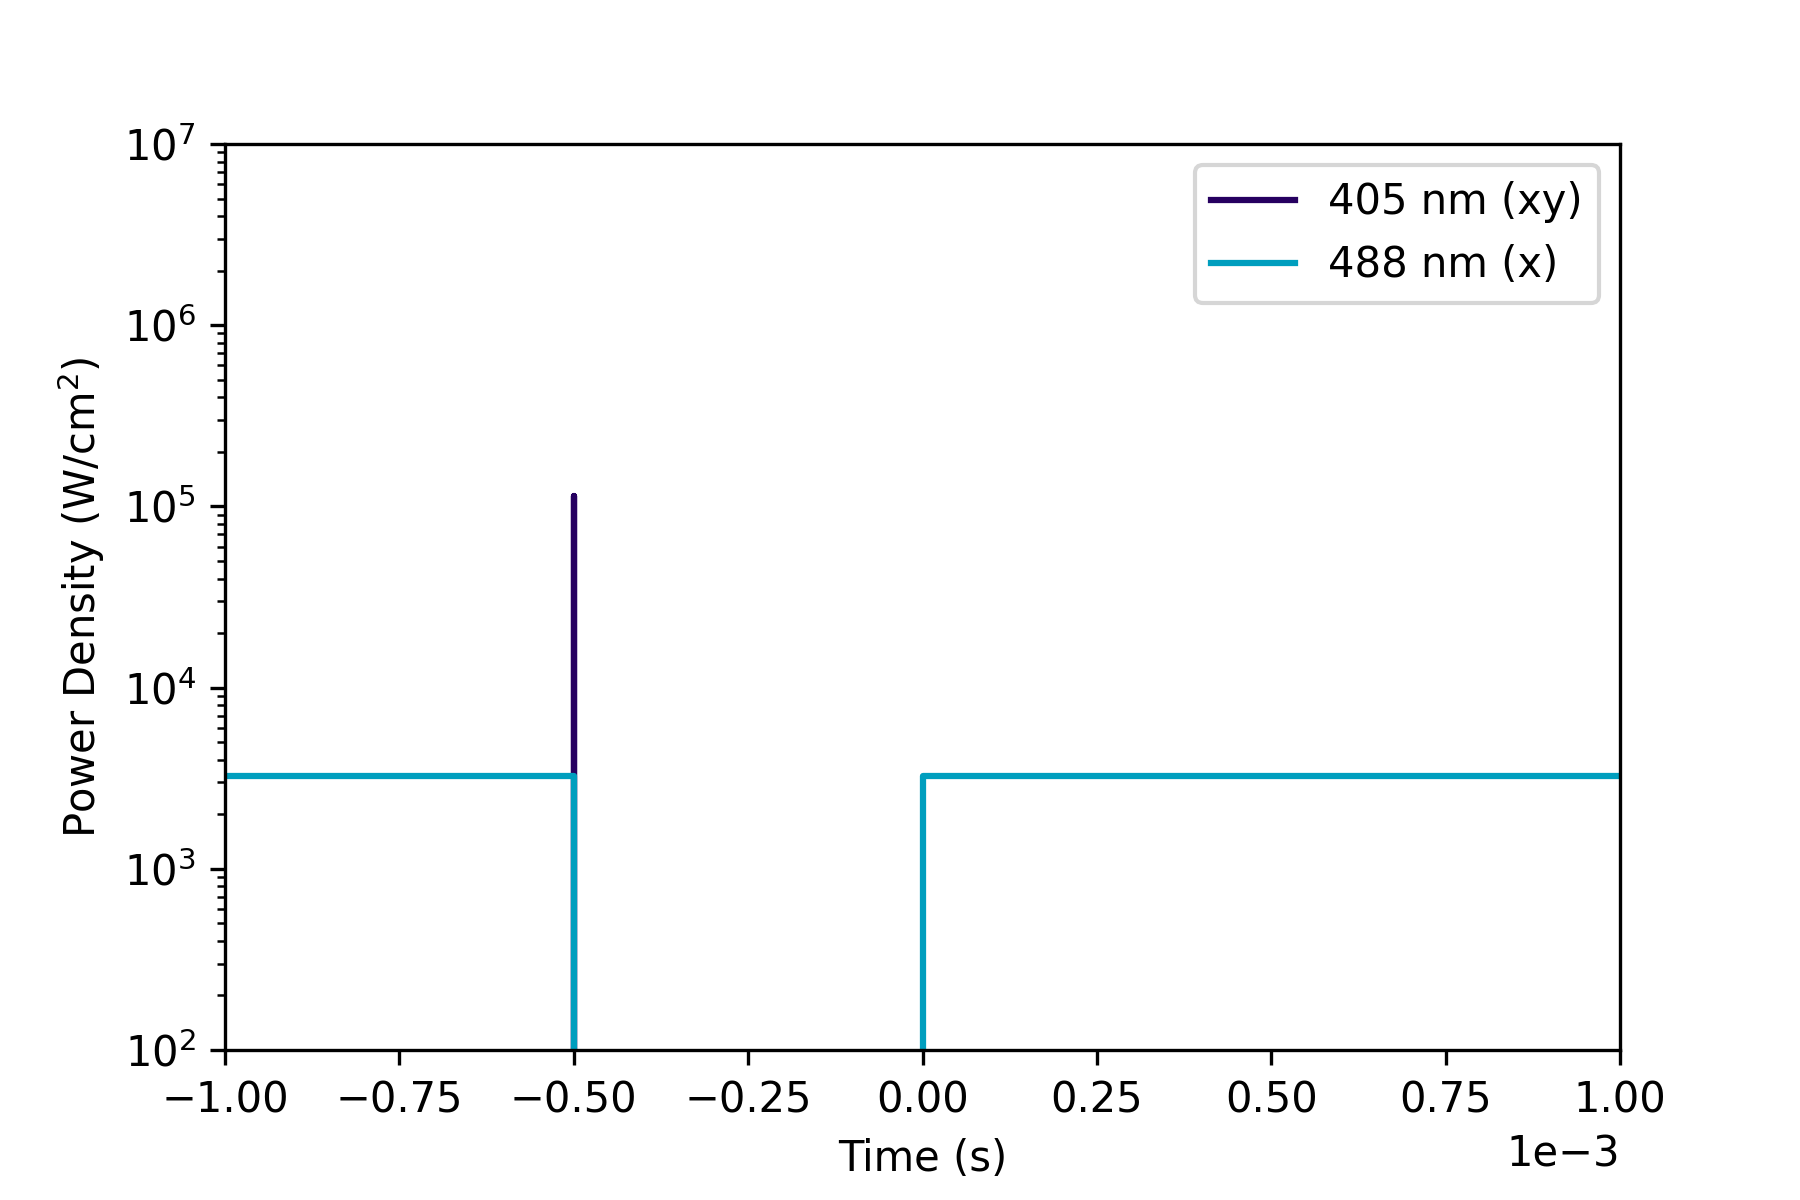
\includegraphics[width=0.8\textwidth]
    {figures/starss2_pulse_scheme.png}
    \caption[Power density used in the simulation of STARSS method 2]
    {Power density of laser beams used in the simulation of STARSS with long-lived states method 2. During the waiting time of 500 $\mu$s, we are not shining light on the sample, letting the on-switching process fully complete.}
    \label{fig:starss2_pulse_scheme}
\end{figure}

% Detectors signal
\begin{figure}[h!]
    \centering
    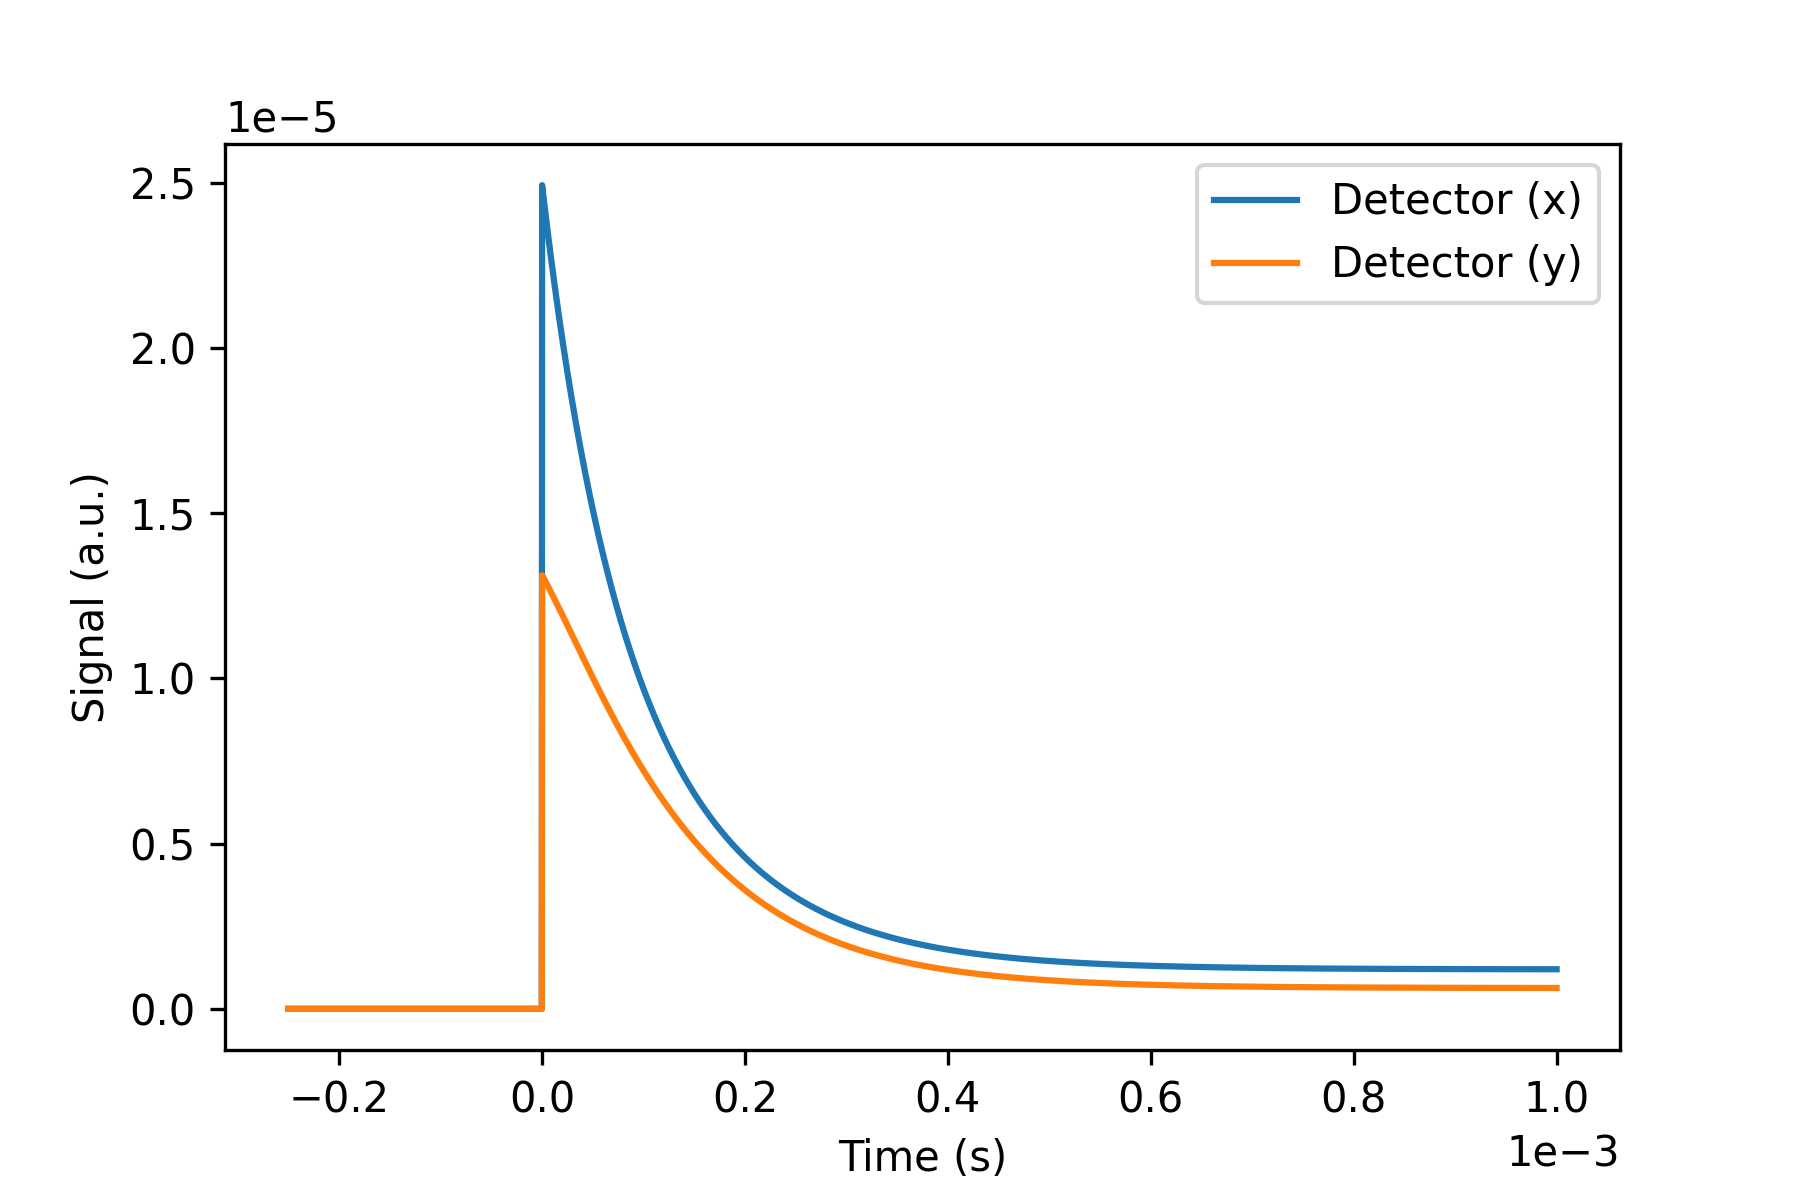
\includegraphics[width=0.8\textwidth]
    {figures/starss2_signal.png}
    \caption[Simulated detector signals of STARSS method 2]
    {Detector signals for parallel (x) and perpendicular (y) channels in the simulation of STARSS with long-lived states method 2 for a rotational diffusion time of 100 $\mu$s and rsEFGP2 fluorophore.}
    \label{fig:starss2_signal}
\end{figure}

The decay of fluorescence anisotropy observed in STARSS method 2 is not easily related to a numerical value of the rotational diffusion coefficient of the system, mainly because the resulting signal is intertwined with photo-physics of the probe. Thus, in order to retrieve the rotational diffusion coefficients, a simulation that includes photo-physical processes must be used.
This require more complex modeling compared to STARSS method 1 where the analogy with the traditional time-resolved fluorescence anisotropy experiment allows for borrowing the theoretical background.
STARSS method 2 experiments have a more convenient on-switching step, that allows saturation of the on-switched population without degradation of the anisotropy signal. This implies that more fluorophores can be on-switched at the same time and higher fluorescence counts can be obtained. Care must be taken if bleaching becomes a relevant factor.

The orientational populations in figure \ref{fig:starss2_sphere_series} complement the description of the experiment with an example for a rotational diffusion time of 100 $\mu$s. At early times a fraction of fluorophores is in the on-state without any preferential orientation, i.e. the first blue sphere is uniformly colored with the shade corresponding to the starting population of on-switched fluorophores. The excited cis-anionic state, represented in green, exhibits a ``cos$^2$'' photo-selection at the beginning of the experiment. This happens because the fluorescence is excited using 488 nm linearly polarized light. The off-switching of fluorophores is more probable when molecules are aligned along X, thus a population \textit{hole} builds-up along X, and the fluorescent photo-selected state will gradually change shape allowing more and more counts to reach the perpendicular detector. At the end of the experiment the system resets itself and is ready for the next pulse sequence.

% Anisotropy
\begin{figure}[h!]
    \centering
    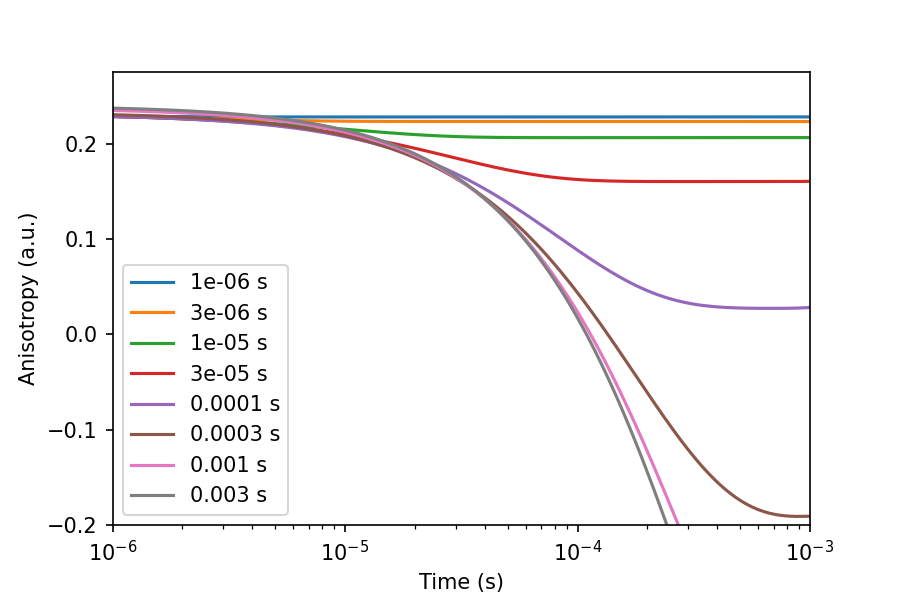
\includegraphics[width=0.8\textwidth]
    {figures/starss2_anisotropy_multiple_decays.png}
    \caption[Simulated fluorescence anisotropy decays of STARSS method 2]
    {Fluorescence anisotropy decays computed for rsEFGP2-labeled systems for STARSS with long-lived states method 2 with rotational diffusion times of 1, 3, 10, 30, 100, 300, 1000, 3000 $\mu$s.}
    \label{fig:starss2_anisotropy}
\end{figure}

% Sphere series
\begin{figure}[h!]
    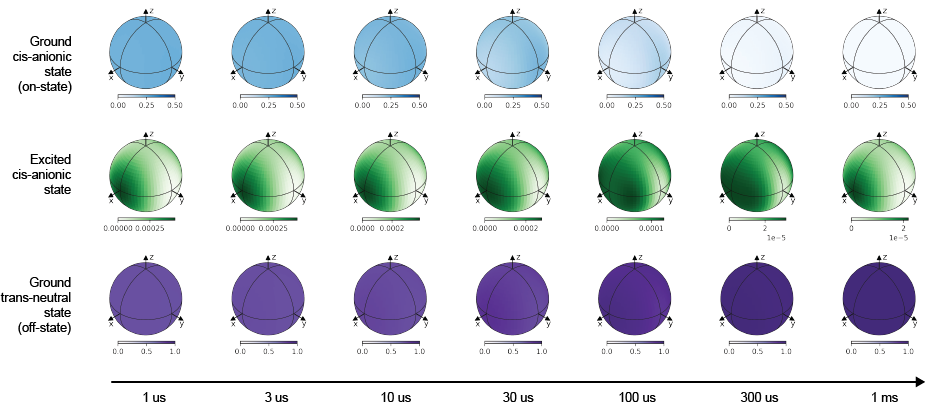
\includegraphics
    [width=\textwidth]
    {figures/starss2_spheres_time_axis.png}
    \caption[Time evolution of orientational probabilities for STARSS method 2]
    {STARSS with long-lived states method 2. Time evolution of orientational probabilities for the ground cis-anionic state (blue), excited cis-anionic state (green), and ground trans-neutral state (purple) for a rotational diffusion time of 100 $\mu$s with rsEGFP2 as fluorophore.}
    \label{fig:starss2_sphere_series}
\end{figure}


\clearpage
%%%%%%%%
\section{STARSS method 3 simulation of experiments}\label{sec:starss_modality3}
In STARSS method 3 an ensemble of rsFPs is on-switched with a couple of very short (50 ns) high power density 405 nm linearly polarized laser pulses. After a waiting time of 200 $\mu$s, the ensemble of on-switched fluorophores is readout with 488 nm circularly polarized light, on a detector without polarization analyzer.
The power density of 405 nm laser pulses is tuned to induce some degree of saturation of the on-switching transition. In this way, when the second pulse arrives at the sample, there will be a different yield of the on-switching process depending on if the fluorophores are still aligned or if they diffused rotationally. Thus, changing the delay between the pulse pair generates a signal that depends on the rotational diffusion coefficient.

The combined fluorescence signal acquired after a pair of on-switching pulses is normalized by dividing by the fluorescence signal obtained from a single on-switching pulse. In this way, the normalized signal ranges between 1 and 2. If the first pulse fully saturates the on-switching process and all the fluorophores are activated regardless of their orientation the signal will be close to 1. In the other limit, when the on-switching is purely linear, the signal will be close to 2, i.e. each 405 nm pulse is on-switching an equal small amount of fluorophores. To obtain the best modulation as a function of the rotational diffusion, the level of saturation should be intermediate and a signal around 1.5 is desirable. When the normalized signal is close to 1 or 2 the rotational diffusion has a small effect.

This experiment has very low hardware requirements on the detection, i.e. there is no need of polarization-sensitive and time-resolved detectors. During the readout with 488 nm light, the fluorescence signal is expected to decay because of the off-switching process. The final observable is the integral of the total counts of the detector during the off-switching curve. An example of off-switching decay after the double pulse activation is reported in Figure \ref{fig:starss3_signal}. STARSS method 3 signals fully neglect the time information of the fluorescence observable during the off-switching process. For this reason it is not necessary to study the evolution of the orientational population along the full pulse scheme.

% Pulse scheme
\begin{figure}[h!]
    \centering
    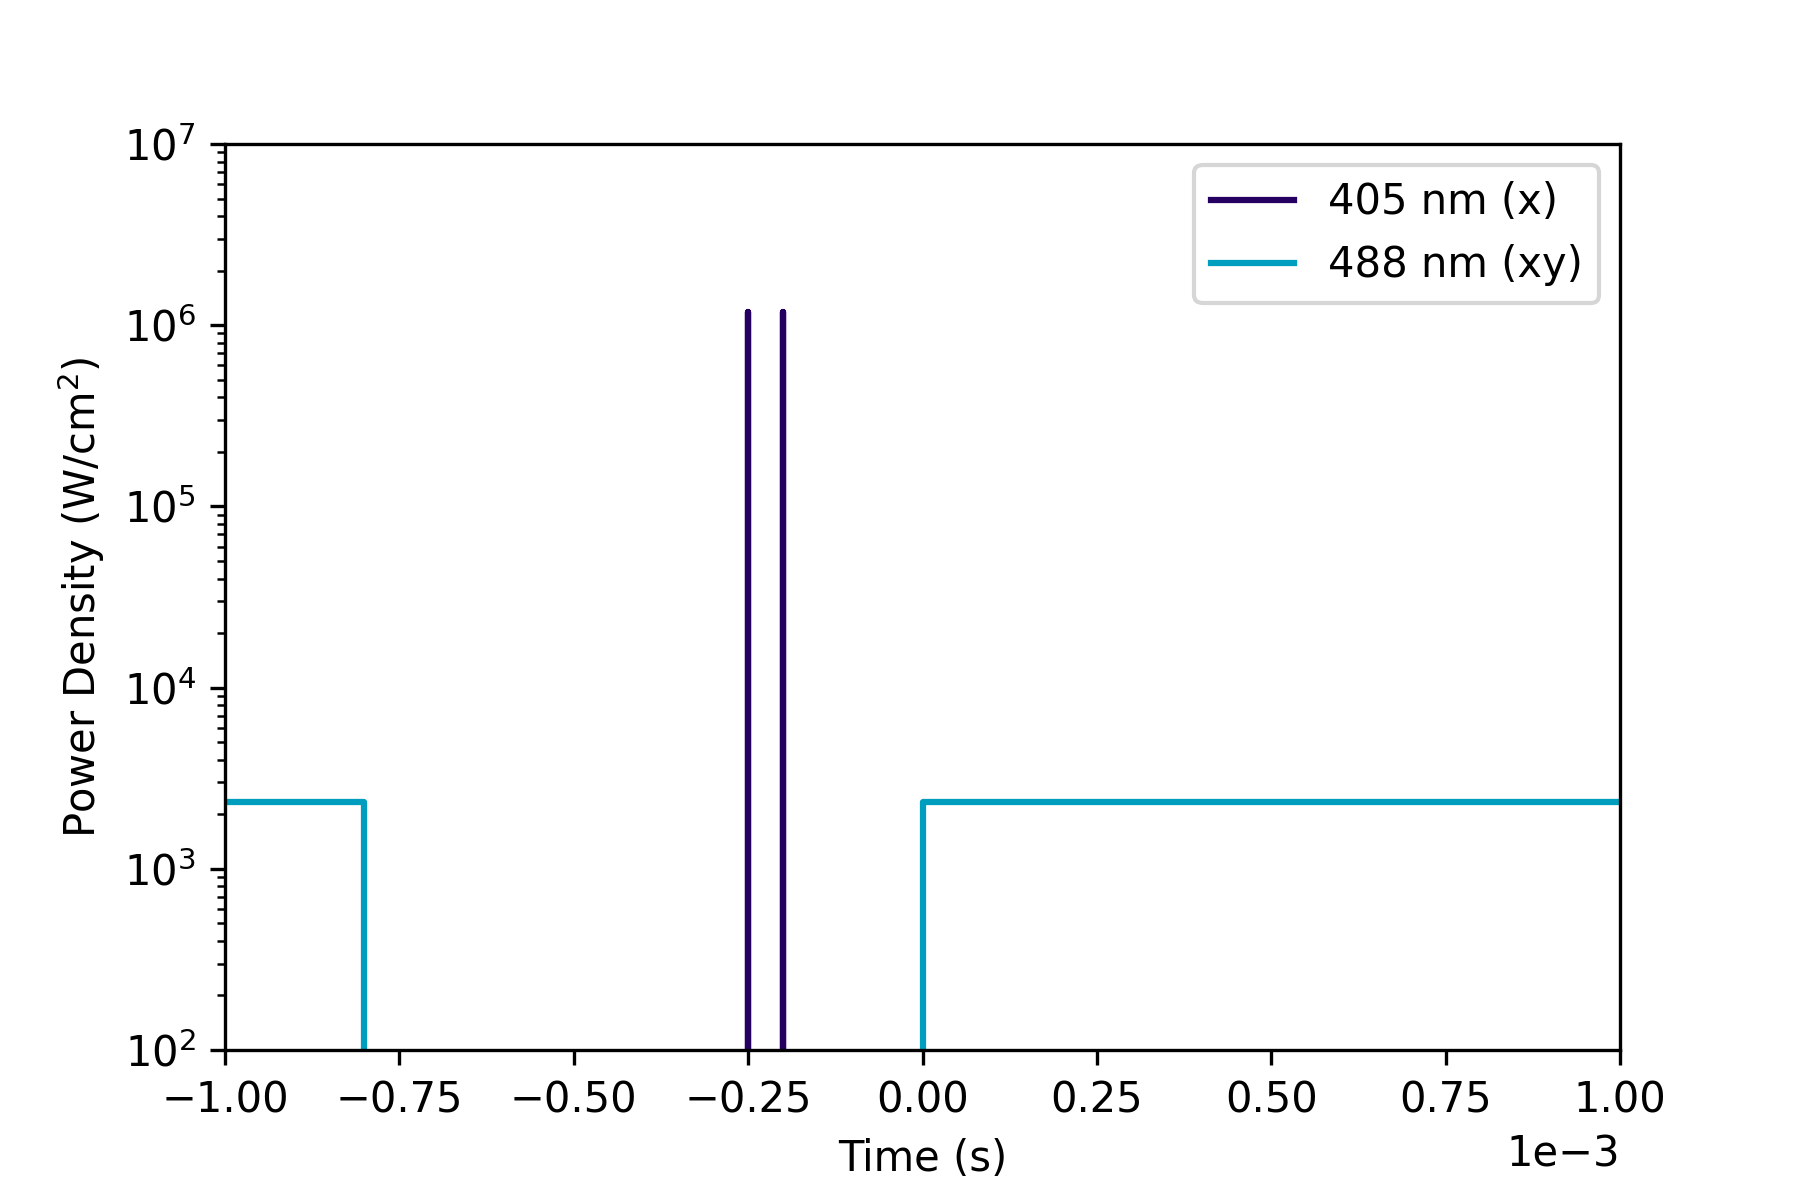
\includegraphics[width=0.8\textwidth]
    {figures/starss3_pulse_scheme.png}
    \caption[Power density used in the simulation of STARSS method 3]
    {Power density of laser beams used in the simulation of STARSS with long-lived states method 3.}
    \label{fig:starss3_pulse_scheme}
\end{figure}

% Detectors signal
\begin{figure}[h!]
    \centering
    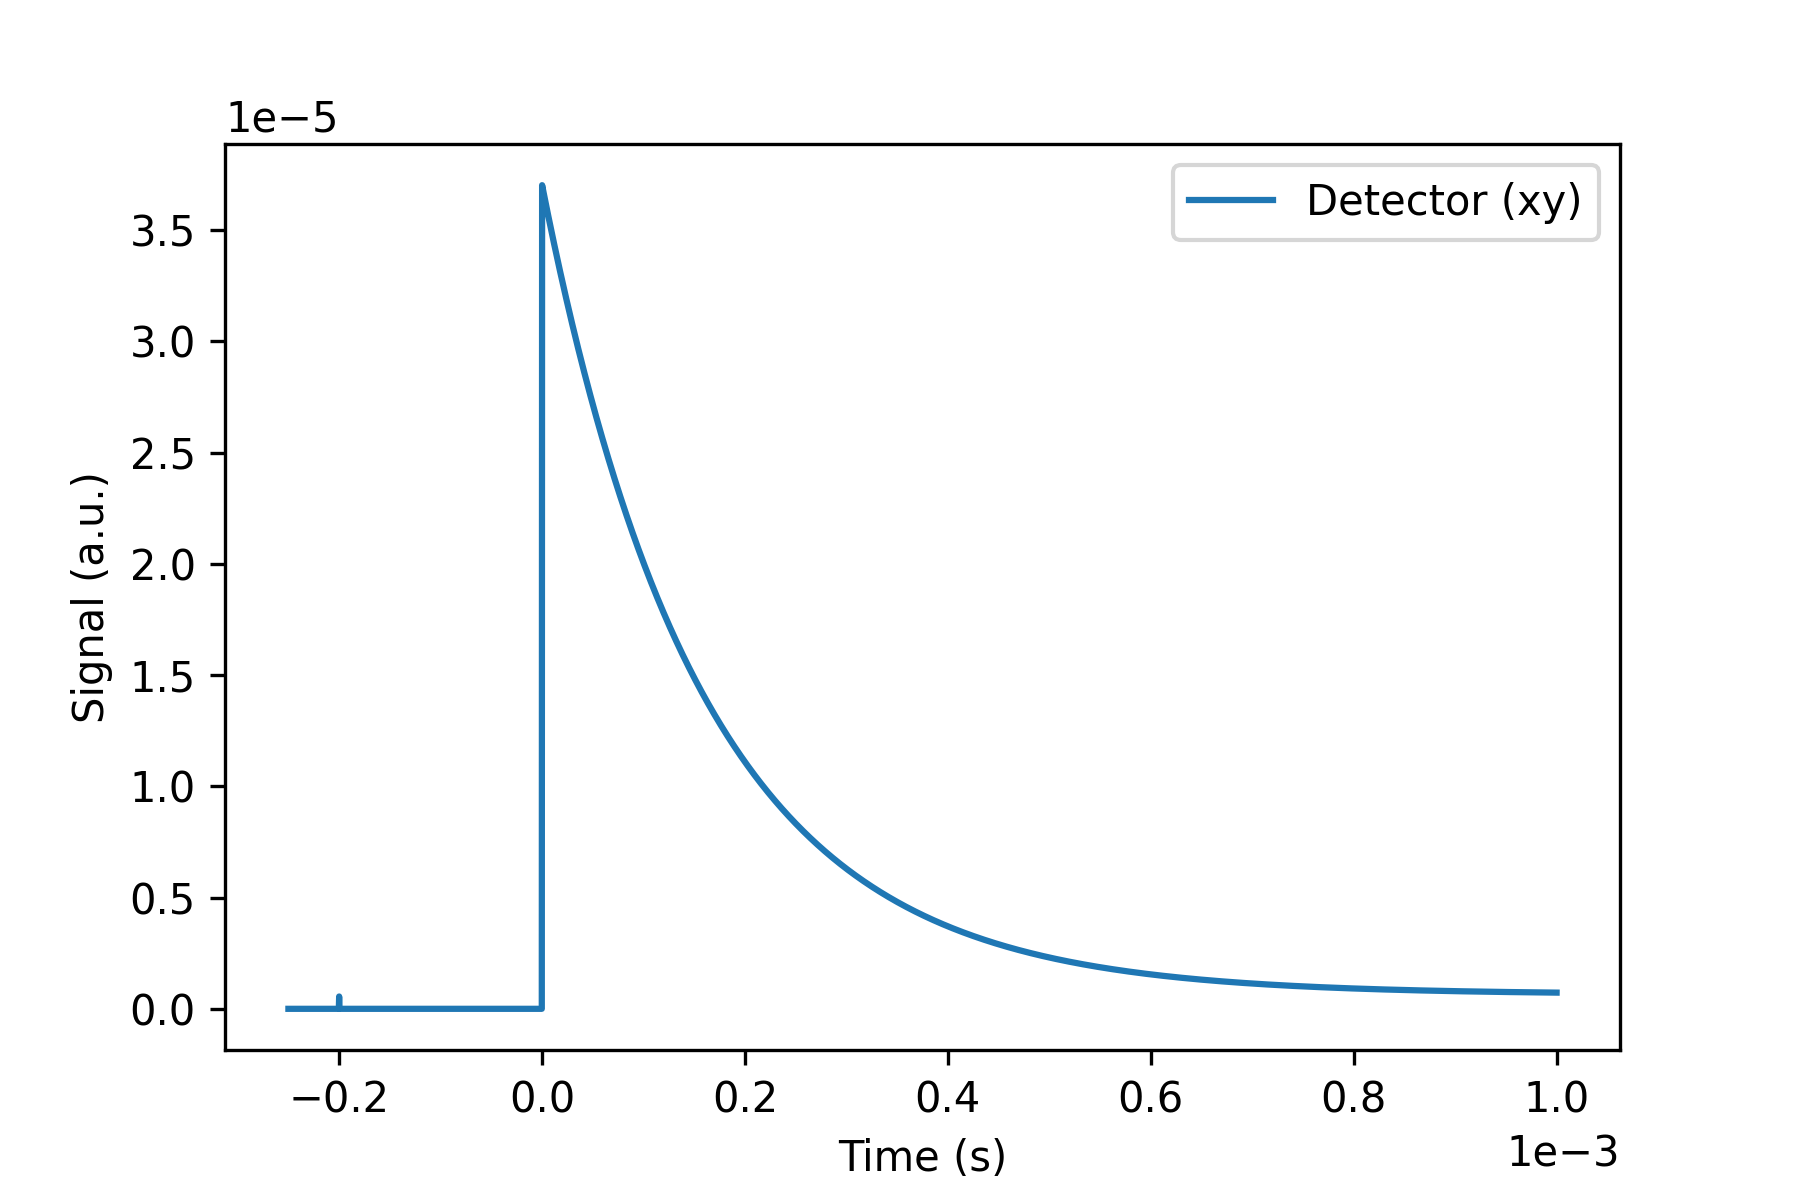
\includegraphics[width=0.8\textwidth]
    {figures/starss3_signal.png}
    \caption[Simulated detector signals of STARSS method 3]
    {Simulated detector signal for a system with a rotational diffusion time of 100 $\mu$s and a delay of 50 $\mu$s between the on-switching pulses of STARSS with long-lived states method 3.}
    \label{fig:starss3_signal}
\end{figure}

% Anisotropy
\begin{figure}[h!]
    \centering
    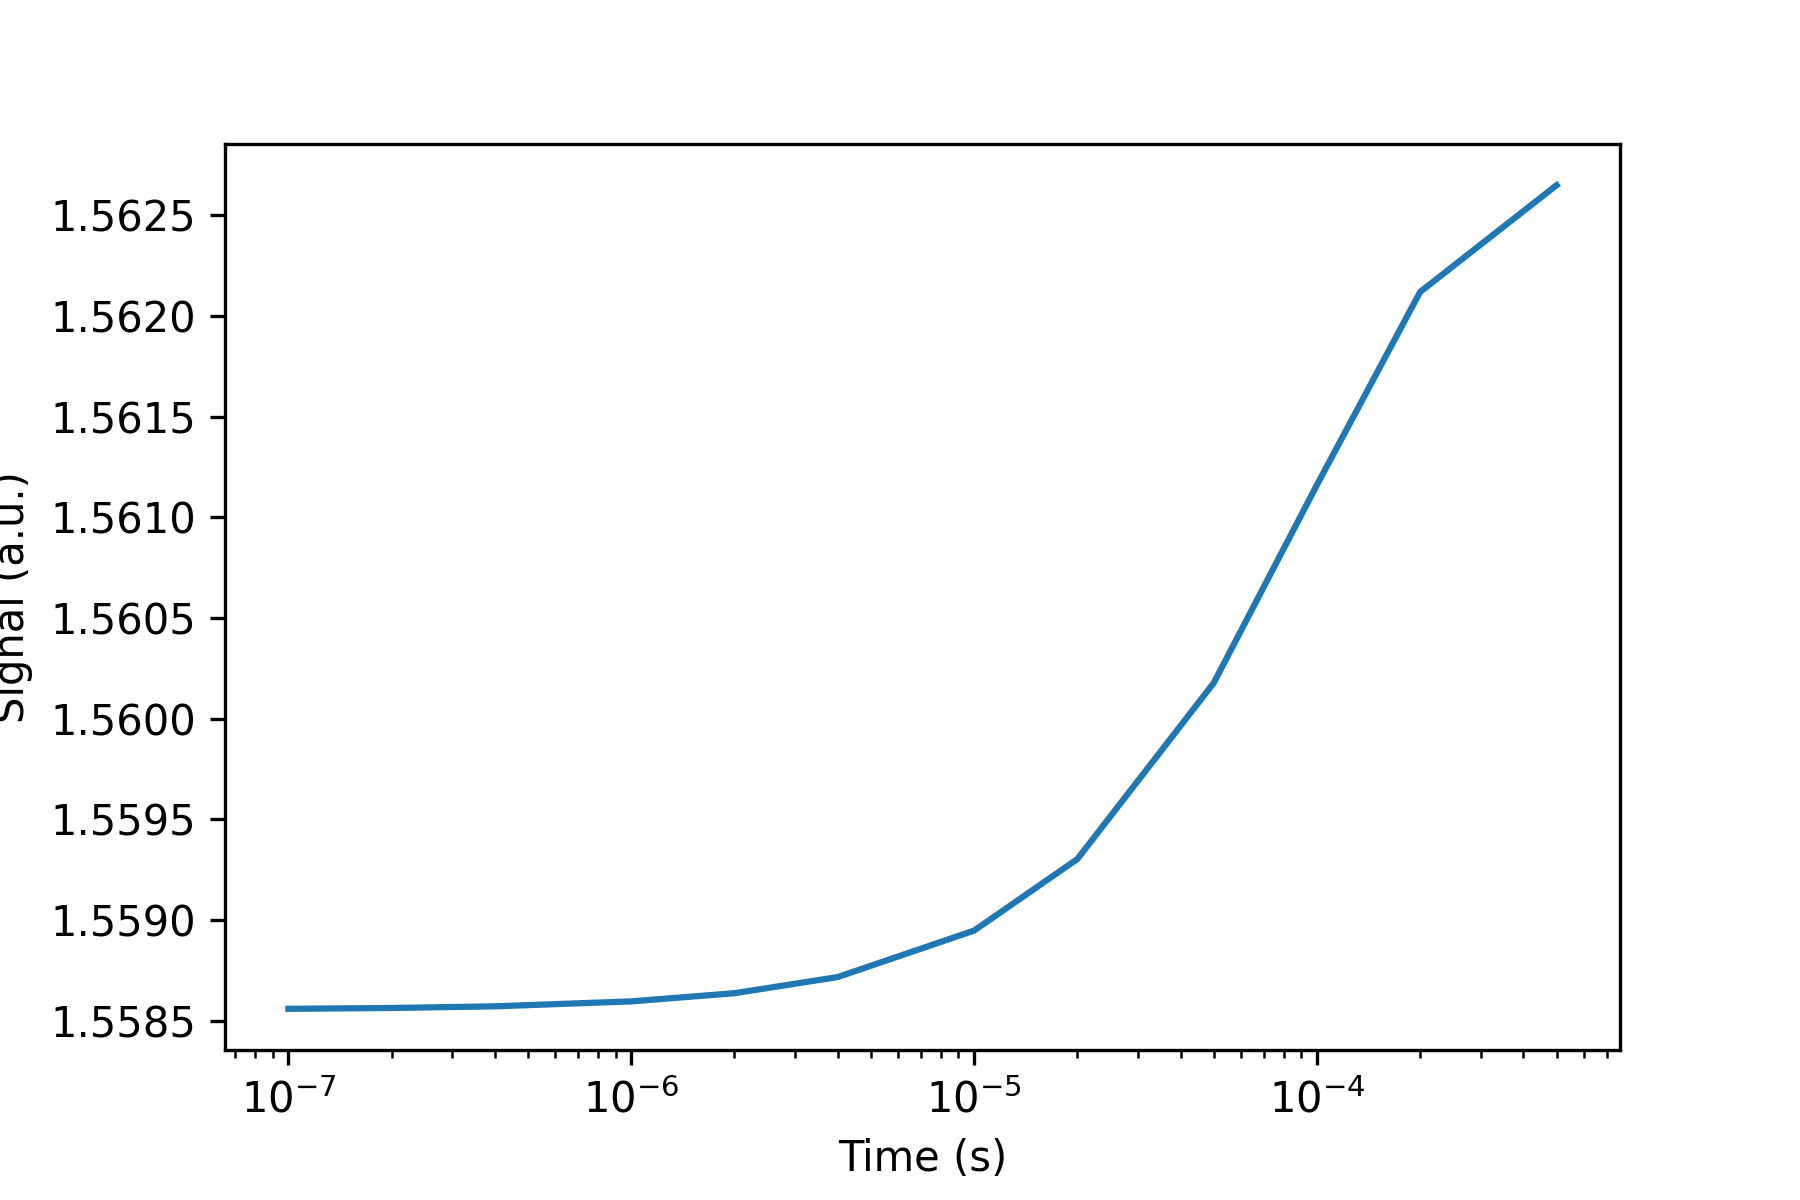
\includegraphics[width=0.8\textwidth]
    {figures/starss3_signals.png}
    \caption[Simulated signals of STARSS method 3]
    {Integrated fluorescence signal computed repeating the simulation of STARSS with long-lived states method 3 as a function of the 405 nm pulse pair delay, which is reported as time axis in the plot. The rotational diffusion time is 100 $\mu$s. The normalization of the signal is done by dividing the total counts obtained with a pulse scheme with two 405 nm pulses by the total counts of a pulse scheme with just one 405 nm pulse, i.e. where the first pulse is not shined on the sample.}
    \label{fig:starss3_signals}
\end{figure}

Repeating the pulse scheme in Figure \ref{fig:starss3_pulse_scheme} for several delay times generated values plotted in Figure \ref{fig:starss3_signals}. An increase of the total fluorescence is observed when the delay between the pulses is increased.
Experimentally a bigger dynamic range for STARSS method 3 experiments was observed, with signals ranging from 1.5 to about 1.7. Nevertheless the shape of the simulated signal capture the same trends observed in experiments (see Figure 2i of main manuscript).


\clearpage
%%%%%%%%%%%%%%%%%%%%%%%%%%%%%%%%%%%%%%%%%%%%%%%%%%%%%%%%%%%%%%%%%%%%%%%%%%%%%%%%
\printbibliography[heading=bibintoc, title={References}]

\end{document}
